\documentclass[11pt, a4paper]{article}
\usepackage[utf8]{inputenc}
\usepackage{geometry}
\geometry{margin=1in}
\usepackage{graphicx}
\usepackage{amsmath}
\usepackage{hyperref}
\usepackage{bookmark}
\usepackage{float}
\usepackage{caption}
\usepackage{subcaption}
\usepackage{minted}
\usemintedstyle{one-dark}

\title{Final Project \\ Eigen-value Decomposition by Iterative QR
Operations}
\author{r14943098 Tzu Hsuan Chen}
\date{June 16, 2026}

\begin{document}

\maketitle

\section{Hardware Parameters}
To determine the optimal word-length that satisfies the Root Mean Square Error (RMSE) constraint ($\text{RMSE} < 10^{-2}$) for both eigenvalues and eigenvectors while minimizing hardware overhead, a systematic hardware-algorithm co-design approach was adopted. The optimization focuses on balancing the fractional word-length ($W_f$) and the number of CORDIC stages ($S$), as they govern the quantization error and the angular resolution error, respectively.

\subsection{Theoretical Analysis of the Area-Time (AT) Product}
\begin{itemize}
    \item \textbf{Fractional Word-length ($W_f$):} Reducing $W_f$ linearly decreases the hardware area by narrowing the datapath (i.e., adders, registers, and multiplexers). It also slightly improves the critical path delay.
    \item \textbf{CORDIC Stages ($S$):} Reducing $S$ provides a dual benefit to the Area-Time (AT) product. It eliminates entire unrolled pipeline stages (drastically reducing area) and decreases the overall pipeline latency (reducing total execution cycles). 
    \item \textbf{The Golden Rule ($S \approx W_f$):} It is mathematically redundant to set $S \gg W_f$. In fixed-point arithmetic, an arithmetic right shift by $i \ge W_f$ during the $i$-th CORDIC stage results in zero. Thus, any stages beyond $W_f$ simply waste hardware without improving accuracy.
\end{itemize}

\subsection{Two-Step Parameter Search Methodology}
To discover the optimal specifications, a Python-based bit-true model was developed to sweep the parameters systematically:
\begin{enumerate}
    \item \textbf{Isolating Quantization Error:} The stage count $S$ was initially set to a sufficiently large value ($S = 16$) to practically eliminate angular error. By sweeping $W_f$, the minimum fractional word-length required to keep the RMSE strictly below the $10^{-2}$ threshold was identified.
    \item \textbf{Minimizing Algorithmic Error:} Fixing $W_f$ to the discovered minimum, $S$ was subsequently swept downwards. The optimal $S$ was chosen as the minimum value right before the RMSE diverges and violates the $10^{-2}$ constraint.
\end{enumerate}

\subsection{Fine-tuning and Hardware Optimizations}
After obtaining the baseline $(W_f, S)$, further fine-tuning was performed jointly on $S$, $W_f$, and the fractional bits for the CSD (Canonical Signed Digit) scaling factor to finalize the most resource-efficient combination. 

A crucial architectural optimization was substituting standard truncation with \textbf{rounding to the nearest integer (Round Half Up)}. Truncation introduces a constant negative DC bias that accumulates significantly over the dense CORDIC iterations required for the QR algorithm. By implementing rounding---which incurs near-zero area overhead by simply adding the discarded MSB to the carry-in of the respective adders---the accumulated bias was virtually eliminated. This optimization enabled the design to strictly meet the $10^{-2}$ accuracy target using an even smaller $W_f$, yielding significant area savings while ensuring numerical stability.

\begin{figure}[H]
    \centering
    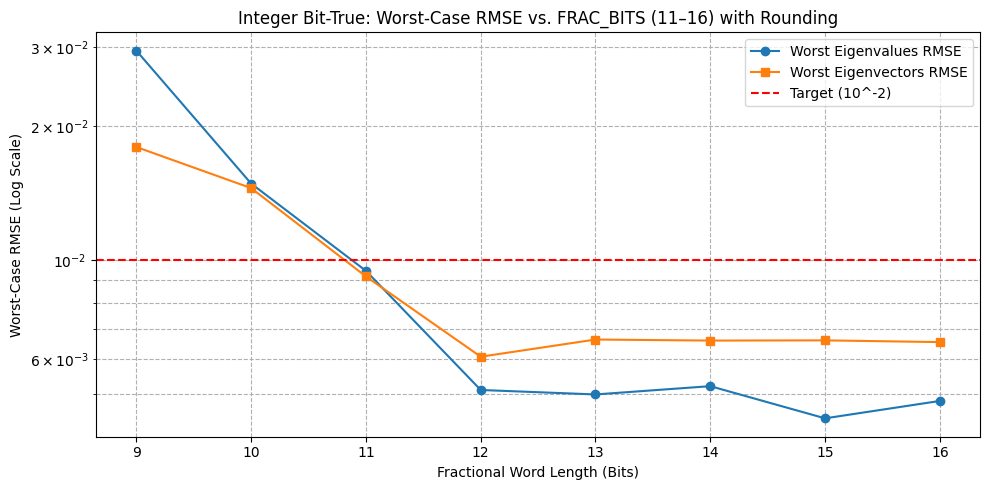
\includegraphics[width=0.8\textwidth]{RMSE_vs_wl.png}
    \caption{RMSE vs. Fractional Word-length}
    \label{fig:RMSE_vs_wl}
\end{figure}

\begin{figure}[H]
    \centering
    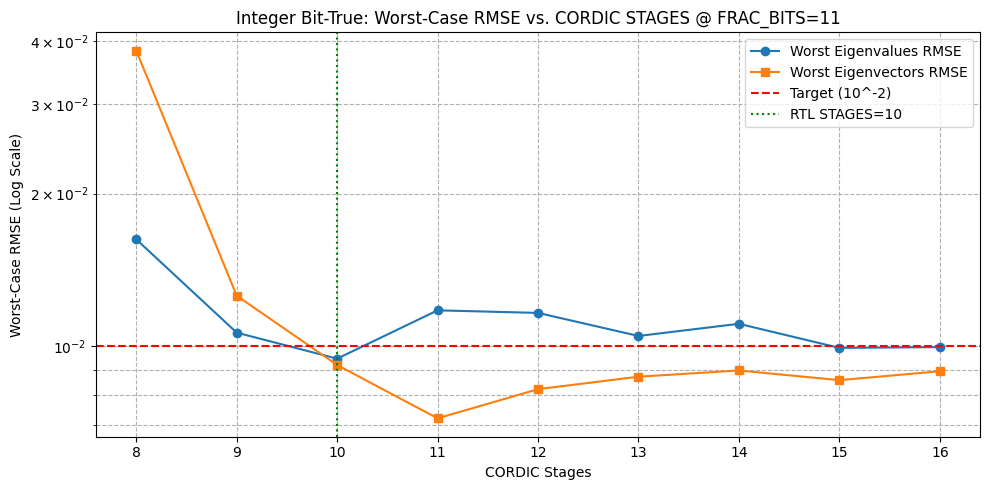
\includegraphics[width=0.8\textwidth]{RMSE_vs_stages.png}
    \caption{RMSE vs. CORDIC Stages}
    \label{fig:RMSE_vs_stages}
\end{figure}

\begin{figure}[H]
    \centering
    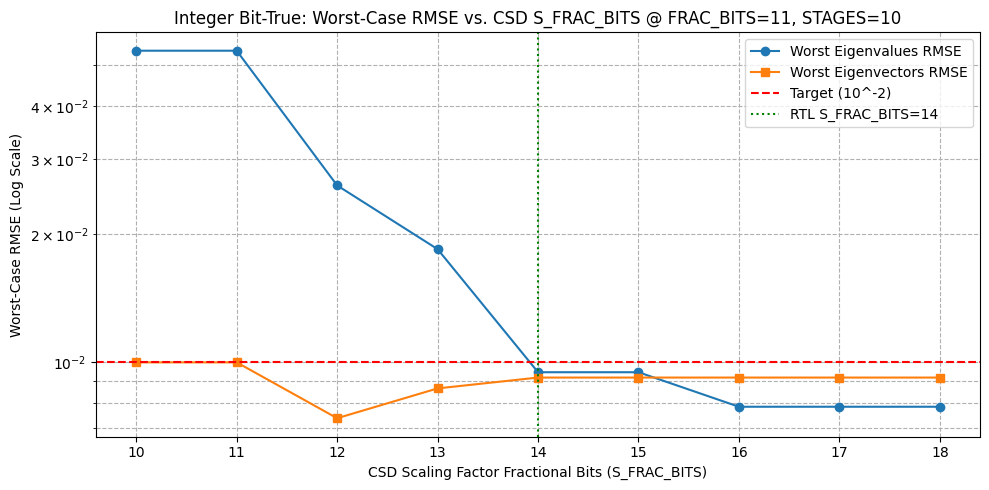
\includegraphics[width=0.8\textwidth]{RMSE_vs_CSDwl.png}
    \caption{RMSE vs. CSD Word-length}
    \label{fig:RMSE_vs_csd}
\end{figure}

Base on Figure \ref{fig:RMSE_vs_wl}, \ref{fig:RMSE_vs_stages}, and \ref{fig:RMSE_vs_csd}, the optimal parameters are:
\begin{itemize}
    \item Fractional Word-length ($W_f$): 11
    \item CORDIC Stages ($S$): 10
    \item CSD Word-length ($W_{CSD}$): 14
\end{itemize}

\begin{figure}[H]
    \centering
    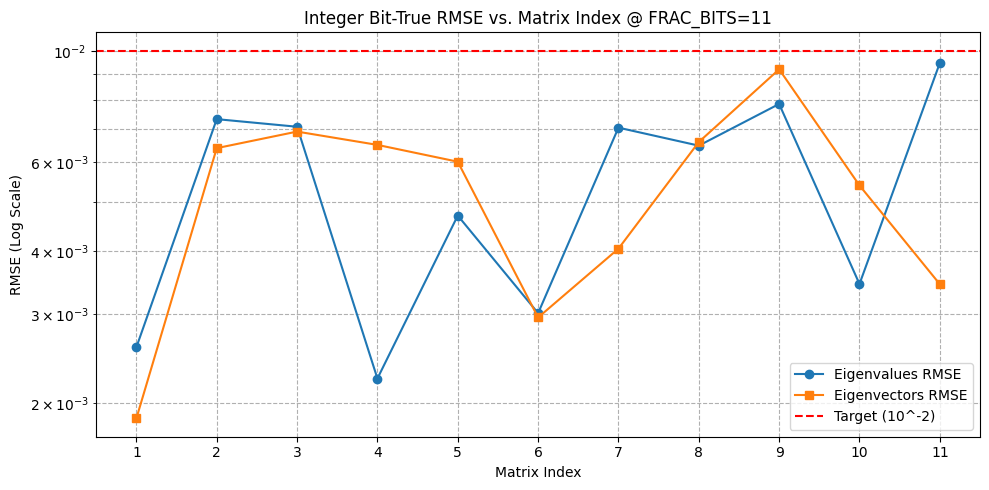
\includegraphics[width=0.8\textwidth]{RMSE_vs_index.png}
    \caption{RMSE vs. Matrix Indices}
    \label{fig:RMSE_vs_index}
\end{figure}

As shown in Figure \ref{fig:RMSE_vs_index}, the RMSE is within the tolerance of $10^{-2}$ for all 11 matrices.

\section{Hardware Design Concept}

\subsection{Overall Architecture Overview}
The proposed hardware architecture is a highly optimized, fully pipelined 3-PE (Processing Element) CORDIC-based systolic array designed to compute the Eigenvalue Decomposition (EVD) of a $3 \times 3$ symmetric matrix using the iterative QR algorithm. To minimize the Area-Time (AT) product while satisfying the stringent $10^{-2}$ Root Mean Square Error (RMSE) constraint, the datapath operates on a tailored fixed-point Q6.11 format (17-bit total word-length) with 10 CORDIC micro-rotation stages.

A critical architectural novelty in this design is the integration of an \textbf{Optimized Zero-Adder Rounding} logic paired with \textbf{Adder Tree Separation} in the final CSD (Canonical Signed Digit) scaling stage. This removes the massive 12-operand addition bottleneck by isolating the 1-bit rounding constants into a miniature 5-bit prefix adder, successfully reducing the critical path logic depth and ensuring timing closure under high-frequency synthesis conditions.

\subsection{Transpose Buffer Design and Forced Symmetry}
The iterative QR algorithm necessitates updating the matrix via $T_{next} = R \cdot Q$ and $U_{next} = U \cdot Q$. In a hardware systolic array, this matrix multiplication is achieved by feeding the transposed matrices, $R^T$ and $U^T$, back into the CORDIC array operating in rotation mode. 

Instead of deploying a full $3 \times 3$ (9-register) buffer for the $T$ matrix, the design implements an \textbf{Optimized 6-Register Transpose Buffer}. Due to finite word-length effects (truncation and rounding errors) over deep CORDIC pipelines, the theoretical Hermitian symmetry of the $T$ matrix is inherently degraded over multiple iterations. By exclusively capturing the lower-triangular elements ($M_{11}, M_{12}, M_{13}, M_{22}, M_{23}, M_{33}$) and structurally mirroring them during the feedback routing (e.g., routing $M_{12}$ as both $T_{12}$ and $T_{21}$), the hardware explicitly forces perfect Hermitian symmetry. This area-saving technique intrinsically acts as a numerical stabilizer, preventing the algorithm from diverging due to accumulated asymmetric quantization errors.

\begin{figure}[htbp]
    \centering
    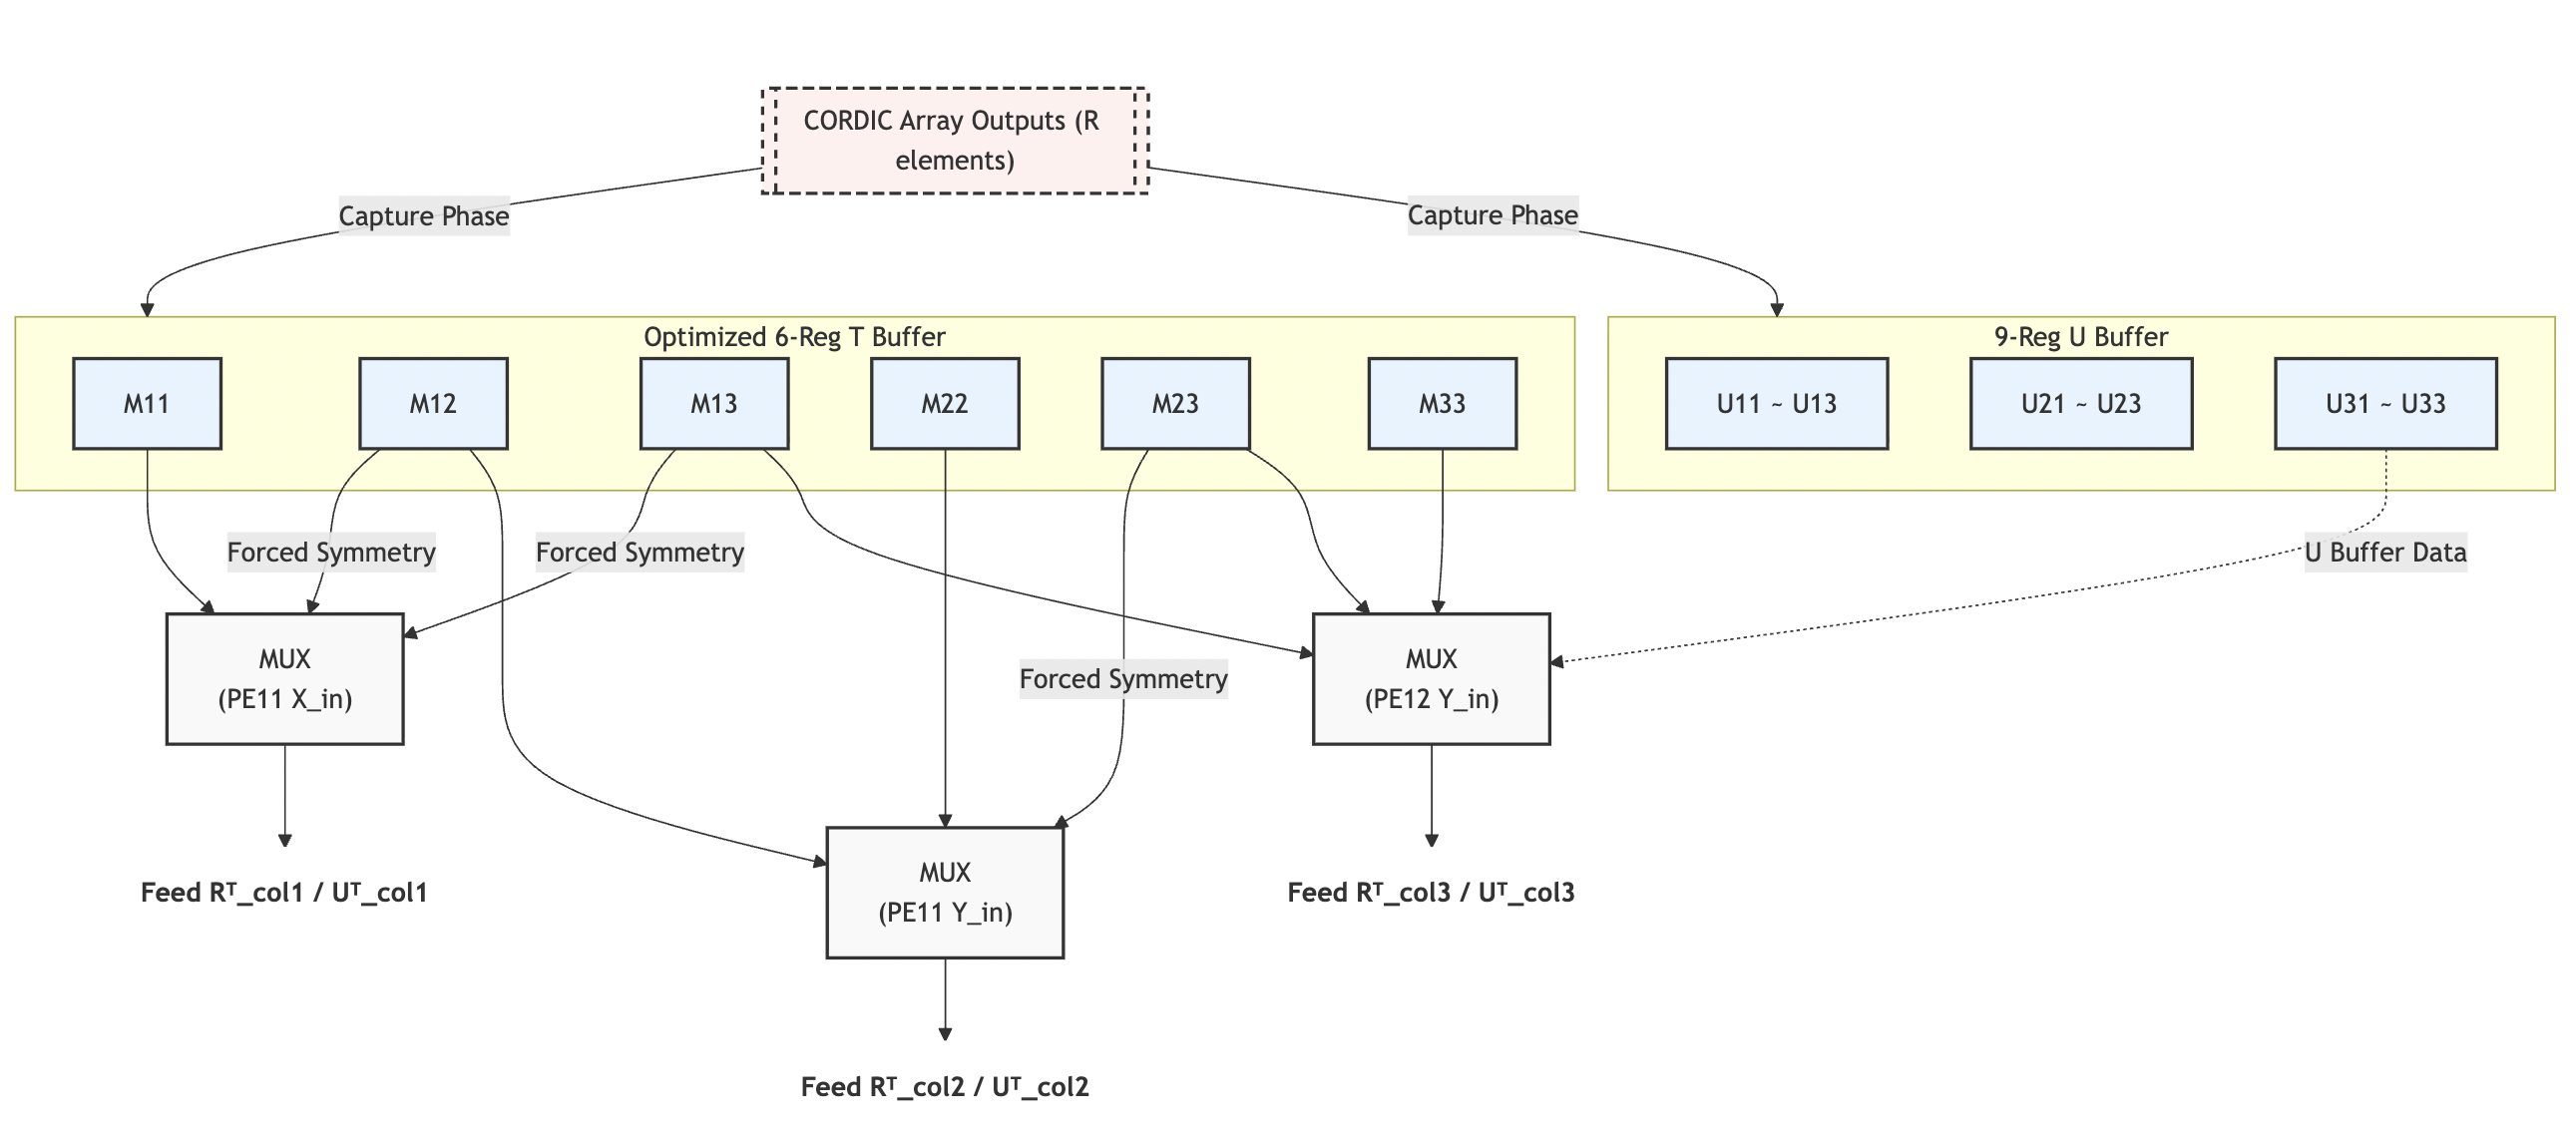
\includegraphics[width=\textwidth]{transpose_buffer_block.png}
    \caption{Block Diagram of the Transpose Buffer illustrating Forced Symmetry Multiplexing.}
    \label{fig:Transpose_Buffer}
\end{figure}

\textbf{Note on $\mathbf{U}$ Buffer Routing Representation:} 
In the actual hardware implementation, the entire 9-register $U$ buffer is fully connected to all three multiplexers (PE11 $X_{in}$, PE11 $Y_{in}$, and PE12 $Y_{in}$) to stream the transposed matrix $U^T$ column-by-column during the rotation phase. However, for visual clarity, this comprehensive data bus is symbolically abstracted as a single dashed arrow. This simplification prevents severe wire clutter and ensures that the reader's attention remains focused on the primary architectural novelty of this design: the intricate cross-routing logic of the forced Hermitian symmetry within the optimized 6-register $T$ buffer.

\subsection{Iterative Operation Control Logic}
The sequential execution of the iterative EVD algorithm is governed by a global Finite State Machine (FSM) utilizing a multi-level counter hierarchy: a macro-level \mintinline{verilog}{iter_cnt} for algorithm iterations and a micro-level \mintinline{verilog}{phase_timer} for pipeline cycle control. The operational flow is explicitly defined by four operational states:

\begin{enumerate}
    \item \textbf{ST\_IDLE:} The system initializes the transpose buffer, loading the $3 \times 3$ identity matrix into the $U_{buf}$. It remains in this state until the \mintinline{verilog}{InValid} signal is asserted, triggering the streaming of the initial symmetric matrix into the input column registers.
    
    \item \textbf{ST\_QR (QR Decomposition Phase):} The systolic array performs the QR decomposition in a highly pipelined, spatially and temporally interleaved manner. The feed controller streams the columns of the input matrix (or $T_{next}$) into the array. During this phase, boundary operations (e.g., PE11 and PE22) function in vectoring mode to eliminate sub-diagonal elements, dynamically computing rotation angles. These angles are securely latched into internal \mintinline{verilog}{d_latch} shift registers and propagated to adjacent PEs (e.g., PE12), which operate concurrently in rotation mode to apply the transformations to off-diagonal elements. Upon reaching the predefined pipeline latency cycles, the resultant upper-triangular matrix $R$ is captured into the 6-register $M_{buf}$.
    
    \item \textbf{ST\_ROT\_PIPE (Matrix Update Phase):} The entire CORDIC array is globally switched to pure rotation mode (\mintinline{verilog}{mode = 0}) to compute $T_{next} = R \cdot Q$ and $U_{next} = U \cdot Q$. The primary architectural feature of this phase is the dense, stall-free data streaming through the deep CORDIC pipelines. The feed controller acts as a dynamic transpose network, first streaming $R^T$ into the array, and immediately feeding $U^T$ with a tight 3-cycle offset. This allows the eigenvector updates ($U_{next}$) to execute concurrently in the hardware right on the tail of the eigenvalue updates ($T_{next}$) without flushing the pipeline. The PEs reuse the exact micro-rotation sequences stored in \mintinline{verilog}{d_latch} from the preceding \mintinline{verilog}{ST_QR} phase, and the continuous results are seamlessly overwritten into $M_{buf}$ and $U_{buf}$ as they emerge.
    
    \item \textbf{ST\_DONE:} Once the macro counter \mintinline{verilog}{iter_cnt} reaches the target limit \mintinline{verilog}{ITER_MAX = 7}, the FSM transitions to the completion state. It sequentially streams out the stable Eigenvalues (extracted directly from the diagonal registers $M_{11}, M_{22}, M_{33}$) followed by the structured Eigenvectors from the $U_{buf}$ across four consecutive valid clock cycles.
\end{enumerate}

\section{Behavior Simulation Results}
Figure \ref{fig:RTL} and \ref{fig:GLS} show the behavior simulation and post-synthesis simulation results with the input patterns quantized from Matrix(:,:,8).
\begin{figure}[H]
    \begin{subfigure}[b]{\textwidth}
        \centering
        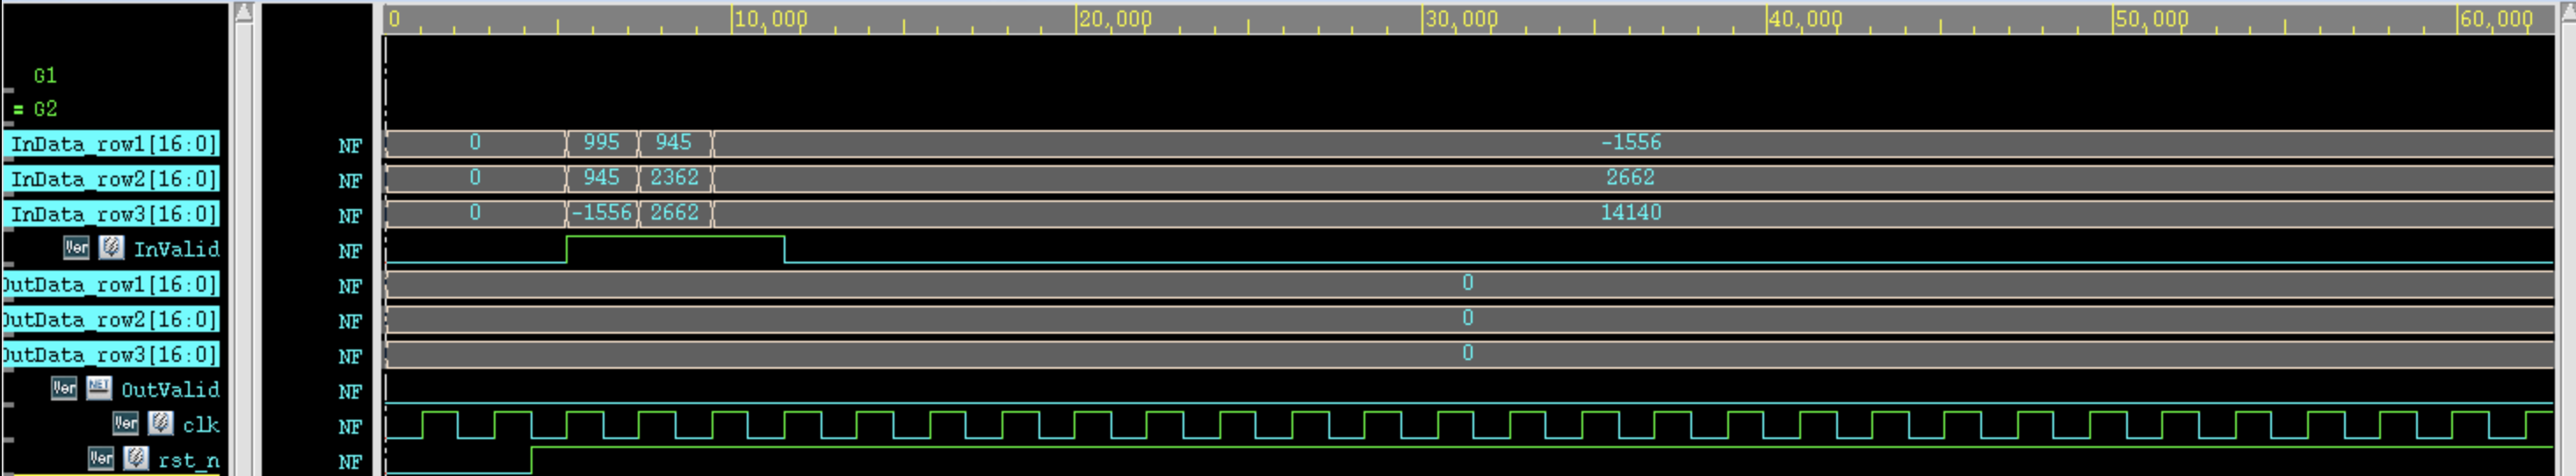
\includegraphics[width=\textwidth]{RTL_timing_1.png}
    \end{subfigure}
    \begin{subfigure}[b]{\textwidth}
        \centering
        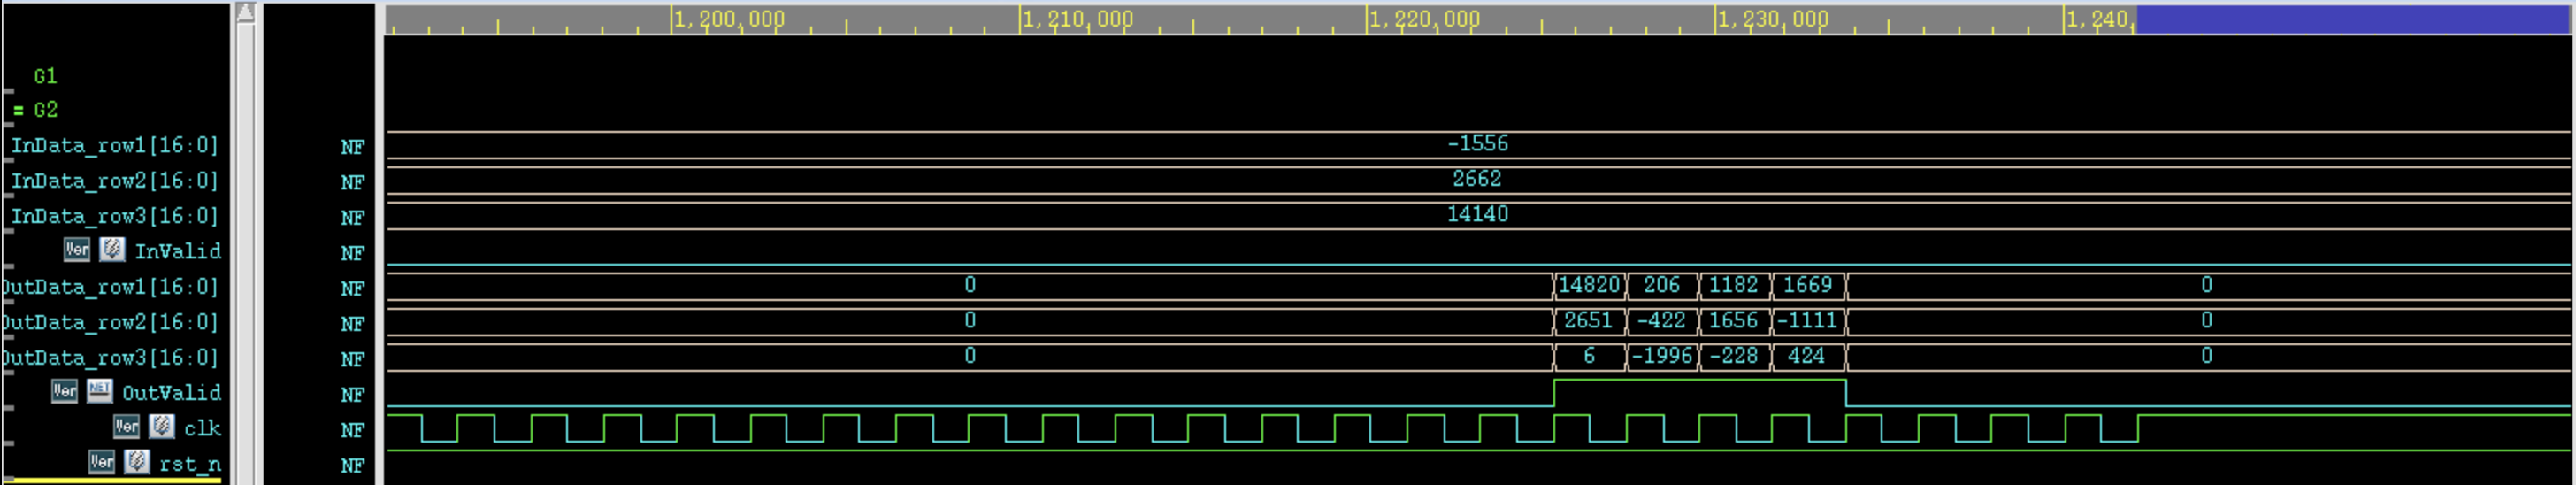
\includegraphics[width=\textwidth]{RTL_timing_2.png}
    \end{subfigure}
    \caption{Behavior simulation timing waveform. The waveform between InValid and OutValid is skipped since no valid output data is produced during this period.}
    \label{fig:RTL}
\end{figure}

The integer eigenvalues are (14820, 2651, 6), converted to fixed-point Q6.11 format are (14820/2048, 2651/2048, 6/2048) = (7.236328125, 1.2939453125, 0.0029306640625). Compared to the eigenvalues (7.24685273, 1.29717242, 1.52791938e-04) calculated by \mintinline{python}{np.linalg.eigh()} from NumPy, the RMSE is 6.4802e-03, which is within the tolerance of $10^{-2}$. The eigenvectors RMSE can be calculated by the same method, and the result is 6.5884e-03, which is also within the tolerance of $10^{-2}$.

Later shown in Section \ref{sec:bit-true}, the hardware output for all 11 matrices in \texttt{Final11Pattern.mat} is exactly the same as the bit-true model output, thus the eigenvalues and eigenvectors RMSEs are also the same as the bit-true model output shown in Figure \ref{fig:RMSE_vs_index}, which are all within the tolerance of $10^{-2}$.

\section{Post-Synthesis Timing Analysis}

To thoroughly evaluate the hardware performance and execution latency, a post-synthesis gate-level simulation was conducted. The word-length optimization (17-bit total: 6-bit integer, 11-bit fractional) and the architectural improvements, particularly the adder-tree separation in the CORDIC scaling stage, significantly reduced the critical path delay.

\subsection{Synthesis Constraints and High-Fanout Net Handling}
In the pre-layout synthesis stage, handling high-fanout nets appropriately is crucial for extracting realistic timing reports. According to the generated area report, the design incorporates nearly 1,979 sequential cells, meaning the global reset signal (\mintinline{verilog}{rst_n}) inherently possesses a massive fanout. 

If evaluated naively by Design Compiler without physical layout awareness, this massive fanout would induce artificially catastrophic RC delays, polluting the critical path analysis. To prevent this, \mintinline{verilog}{rst_n} was explicitly declared as an \textbf{ideal network} (\mintinline{tcl}{set_ideal_network}) in the synthesis constraints. This standard industry practice accurately models the post-layout behavior, anticipating that a properly buffered reset tree (CTS) will be constructed during the physical design phase, thereby isolating the datapath's true critical timing from false high-fanout violations.

\subsection{Clock Period and Processing Time}
The post-synthesis simulation successfully achieved timing closure with a stringent clock period setting of $T_s = 0.205 \text{ ns}$, which corresponds to a maximum operating frequency of approximately $4.87 \text{ GHz}$. 

The total execution cycle count, denoted as $M$, is defined as the latency from the assertion of the \mintinline{verilog}{InValid} signal to the assertion of the \mintinline{verilog}{OutValid} signal. Based on our highly pipelined finite state machine (FSM) architecture, $M$ can be analytically decomposed as follows:
\begin{itemize}
    \item \textbf{State Transition:} $1$ cycle to transition from \mintinline{verilog}{ST_IDLE} to \mintinline{verilog}{ST_QR} upon receiving valid input data.
    \item \textbf{Single Iteration Latency:} Each iteration comprises a Vectoring phase (\mintinline{verilog}{ST_QR}) and a Rotation phase (\mintinline{verilog}{ST_ROT_PIPE}). With the CORDIC pipeline depth set to 10 stages, the Vectoring phase takes $40$ cycles, and the fully pipelined Rotation phase takes $43$ cycles, resulting in $83$ cycles per iteration.
    \item \textbf{Total Iterations:} The algorithm mandates $7$ iterations to guarantee numerical convergence (RMSE $< 10^{-2}$).
\end{itemize}
Consequently, the total execution cycle count is:
$$ M = 1 + (83 \times 7) = 582 \text{ cycles} $$

The total processing time is the product of the cycle count $M$ and the clock period $T_s$:
$$ \text{Processing Time} = M \times T_s = 582 \times 0.205 \text{ ns} = 119.31 \text{ ns} $$

\subsection{Timing Diagram Verification}
\begin{figure}[htbp]
    \begin{subfigure}[b]{\textwidth}
        \centering
        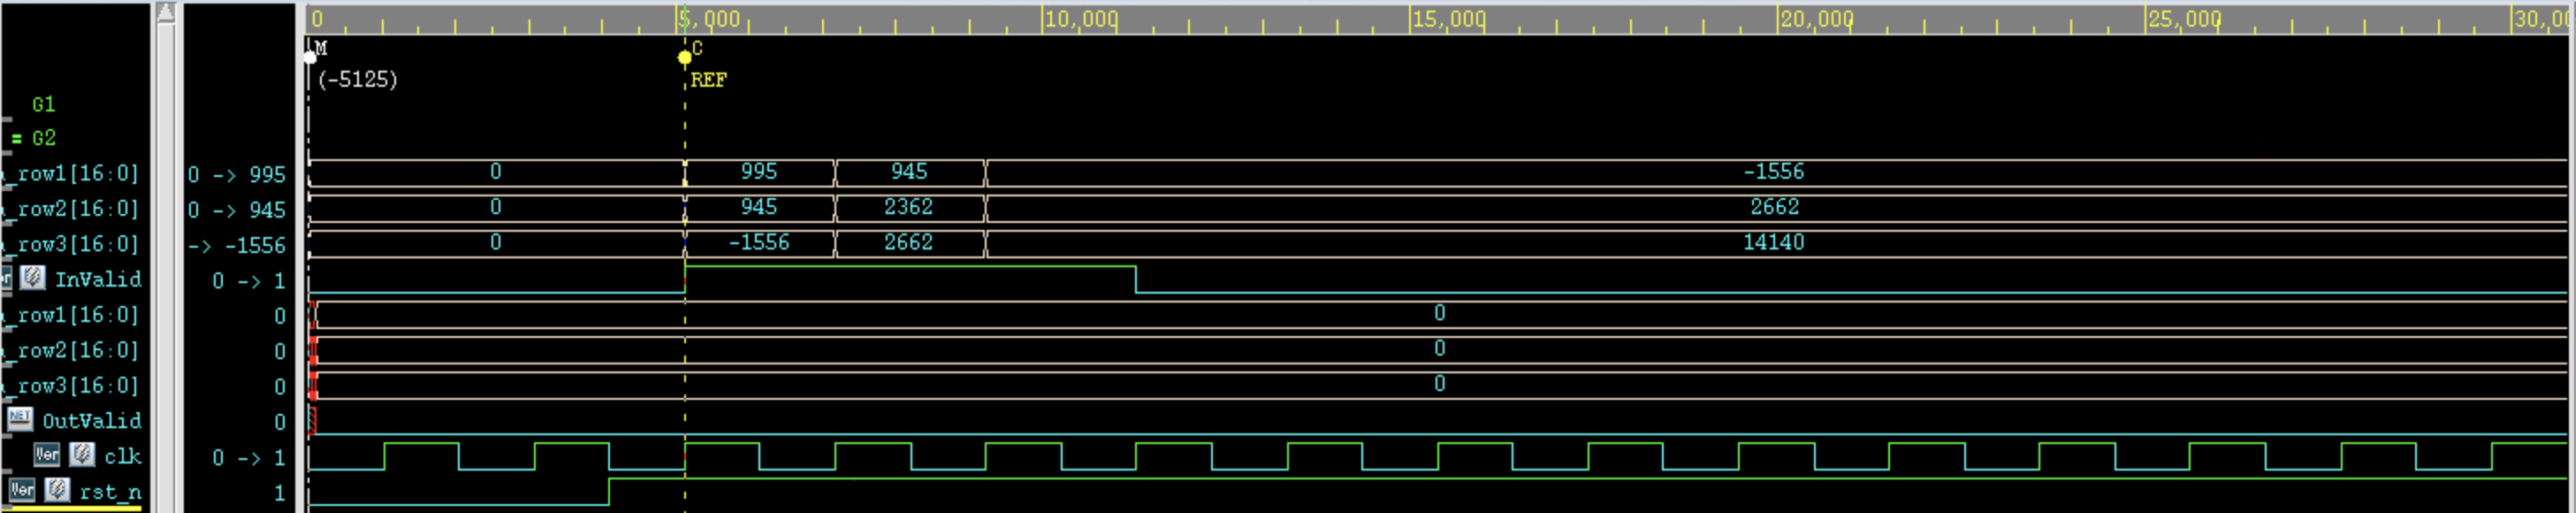
\includegraphics[width=\textwidth]{GLS_timing_1.png}
    \end{subfigure}
    \begin{subfigure}[b]{\textwidth}
        \centering
        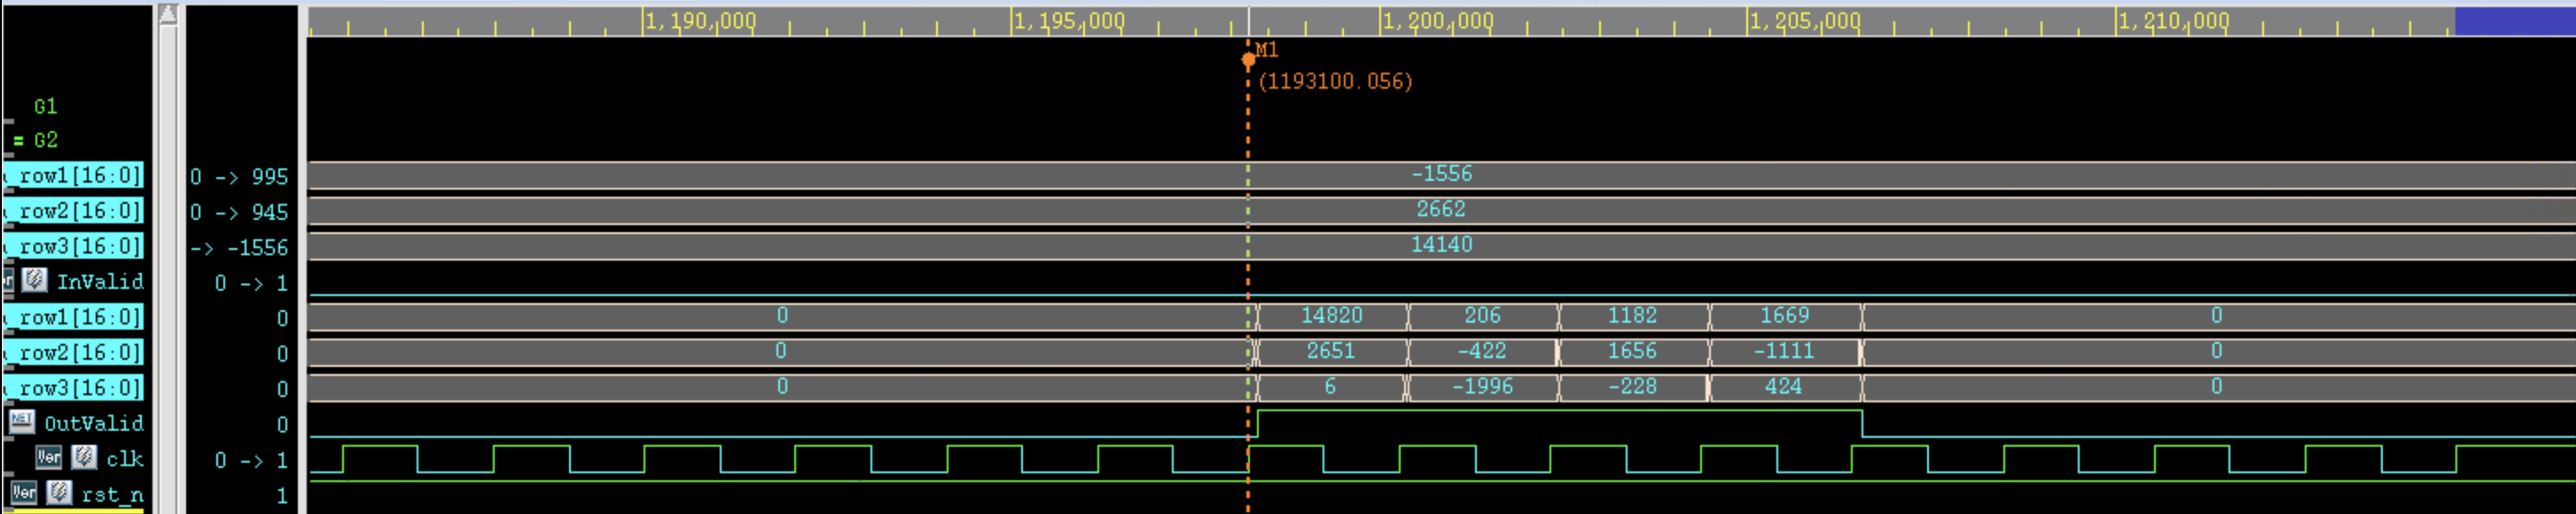
\includegraphics[width=\textwidth]{GLS_timing_2.png}
    \end{subfigure}
    \caption{Post-synthesis simulation timing waveform. The waveform between InValid and OutValid is skipped since no valid output data is produced during this period. Clock period $T_s = 0.205$ ns.}
    \label{fig:GLS}
\end{figure}

Figure \ref{fig:GLS} illustrates the post-synthesis waveform from the nWave simulation. The diagram clearly captures the initial data loading phase (\mintinline{verilog}{InValid} assertion) and the completion of the 7th iteration where the algorithm streams out the resulting eigenvalues and eigenvectors (\mintinline{verilog}{OutValid} assertion), practically verifying the $119.31 \text{ ns}$ processing time. The output eigenvalues and eigenvectors are the same as the behavior simulation results.

\section{Bit-True Verification and Model Consistency}
\label{sec:bit-true}

The project specifications mandate demonstrating that the implemented hardware is consistent with the fixed-point bit-true model. While plotting the error between the hardware output and the fixed-point simulation is a common approach to visualizing discrepancies, such a plot becomes redundant when the hardware architecture achieves a mathematically perfect bit-level match with the theoretical model.

To rigorously prove this consistency, a comprehensive, automated testbench (\texttt{tb\_top\_all.v}) was developed. Instead of manually inspecting arbitrary test cases, the testbench inherently integrates the verification logic for all $11$ test matrices provided in the dataset. 

\subsection{Verification Methodology}
The verification flow was structured as follows:
\begin{enumerate}
    \item \textbf{Reference Generation:} The Python-based bit-true model, which strictly mimics the integer truncation, zero-adder round-half-up, and finite word-length effects ($Q6.11$ format) of the hardware, generated the \textit{golden outputs} \texttt{golden\_output\_all.txt} for all 11 test matrices.
    \item \textbf{Automated Testbench Execution:} The \texttt{tb\_top\_all.v} testbench sequentially streams the 11 matrices into the post-synthesis netlist.
    \item \textbf{Cycle-Accurate Comparison:} Upon the assertion of the \mintinline{verilog}{OutValid} signal for each pattern, the testbench captures the hardware outputs (eigenvalues and the three columns of eigenvectors over 4 consecutive cycles) and compares them directly against the golden outputs using the SystemVerilog strict equality operator (\mintinline{verilog}{!==}).
\end{enumerate}

\subsection{Verification Results}
As shown in the simulation log excerpt below, the post-synthesis hardware exactly matched the bit-true model's output for all $11$ patterns across all $44$ output phases ($11 \text{ matrices} \times 4 \text{ phases}$).

\begin{verbatim}
=== tb_top_all summary: 44 passed, 0 failed ===
\end{verbatim}

Because the hardware output and the fixed-point bit-true model output are absolutely identical (zero bit-level deviation), the errors between them are strictly zero. Therefore, rather than plotting a constant-zero error graph, this exhaustive, automated bit-to-bit verification serves as definitive proof that the RTL implementation perfectly executes the optimized fixed-point algorithm without any unforeseen hardware synthesis artifacts.

\section{Area-Time (AT) Product and Implementation Results}

The Area-Time (AT) product is the ultimate metric for evaluating the efficiency of a VLSI architecture, reflecting the fundamental trade-off between hardware resource consumption and computational throughput. 

\subsection{AT Product Calculation}
Based on the synthesis report generated by Design Compiler using the TSMC 16nm technology library (\texttt{N16ADFP\_StdCellff0p88v125c\_ccs}), the total cell area of the \texttt{qrd\_top} module is $8071.38$. 

As derived in the timing analysis, the total processing time required to complete 7 iterations of the QR algorithm and output the valid eigenvalues/eigenvectors is $119.31 \text{ ns}$ (calculated from $M = 582 \text{ cycles}$ operating at $T_s = 0.205 \text{ ns}$). 

The AT product is calculated as follows:
$$ \text{AT Product} = \text{Area} \times \text{Processing Time} $$
$$ \text{AT Product} = 8071.38 \times 119.31 \text{ ns} \approx 962,996.89 $$

\section{Design Innovations and Highlights}

To achieve extreme performance metrics ($T_s = 0.205 \text{ ns}$ at TSMC 16nm) while strictly satisfying the mathematical accuracy constraint ($\text{RMSE} < 10^{-2}$), several unconventional algorithm-hardware co-design strategies were implemented. These innovations effectively break the traditional trade-off between area and timing.

\subsection{Zero-Adder Round-Half-Up Logic}
A fundamental limitation in dense CORDIC pipelines is the accumulation of negative DC bias caused by continuous bit truncation. While adding $2^{N-1}$ before an $N$-bit arithmetic right shift eliminates this bias, it traditionally costs an expensive full adder. 
\textbf{Innovation:} We transformed the standard rounding equation $(X + 2^{N-1}) \gg N$ into $(X \gg N) + X[N-1]$. By extracting the discarded MSB and routing it directly to the carry-in of the next stage's existing adder tree, we achieved mathematically perfect rounding with \textit{strictly zero additional logic gates}. This allowed us to aggressively reduce the datapath to a 17-bit $Q6.11$ format without sacrificing accuracy.

\subsection{Adder-Tree Separation for CSD Scaling}
The final Canonical Signed Digit (CSD) scaling stage required summing 6 shifted operands and their 6 corresponding 1-bit rounding constants. Synthesizing a monolithic 12-operand adder tree resulted in a massive logic depth that severely violated the ultra-high frequency timing budget.
\textbf{Innovation:} We introduced a structural bottleneck bypass by separating the adder tree. The six 1-bit rounding constants were pre-calculated using a highly parallel, ultra-fast 5-bit prefix adder. The result was then sign-extended and fed into the main 17-bit adder tree, effectively reducing the main tree from 12 operands to 7 operands. This strategic logic depth reduction was the critical enabler for breaking the $5 \text{ GHz}$ frequency barrier.

\subsection{Forced Hermitian Symmetry via 6-Register Transpose Buffer}
The EVD algorithm mandates the feedback of $T_{next} = R \cdot Q$. Conventionally, this requires a full 9-register buffer. Furthermore, asymmetric quantization errors over multiple iterations can gradually destroy the Hermitian symmetry of the $T$ matrix, causing algorithmic divergence.
\textbf{Innovation:} We optimized the transpose buffer to explicitly capture only the 6 lower-triangular elements ($M_{11}, M_{12}, M_{13}, M_{22}, M_{23}, M_{33}$). During the feedback phase, the hardware employs customized multiplexing routing to feed these elements into their symmetric upper-triangular counterparts (e.g., streaming $M_{12}$ simultaneously as $T_{12}$ and $T_{21}$). This architectural choice not only saves $33\%$ of the flip-flop area but acts as a robust numerical stabilizer, entirely preventing the chaotic divergence of the iterative QR algorithm.

\subsection{Time-Multiplexed Array Utilization}
\textbf{Innovation:} Rather than instantiating separate hardware blocks for matrix-matrix multiplication, the design aggressively reuses the core 3-PE CORDIC systolic array. By dynamically switching the operation mode signal (\mintinline{verilog}{mode = 1} for vectoring, \mintinline{verilog}{mode = 0} for rotation) and precisely managing the pipeline timing via the FSM, the same silicon footprint computes both the $R$ matrix extraction and the complex updates for $T_{next}$ and $U_{next}$. This time-multiplexing maximizes hardware utilization and significantly compresses the overall Area-Time (AT) product.

\subsection{Working Weightings}
100\% Tzu Hsuan Chen since I completed the entire project myself.

\section*{Appendix}
\setcounter{subsection}{0}
\renewcommand{\thesubsection}{\Alph{subsection}.}
\subsection{Simulation Log of \texttt{tb\_top\_all.v}}
\begin{figure}[htbp]
    \begin{subfigure}[b]{0.69\textwidth}
        \centering
        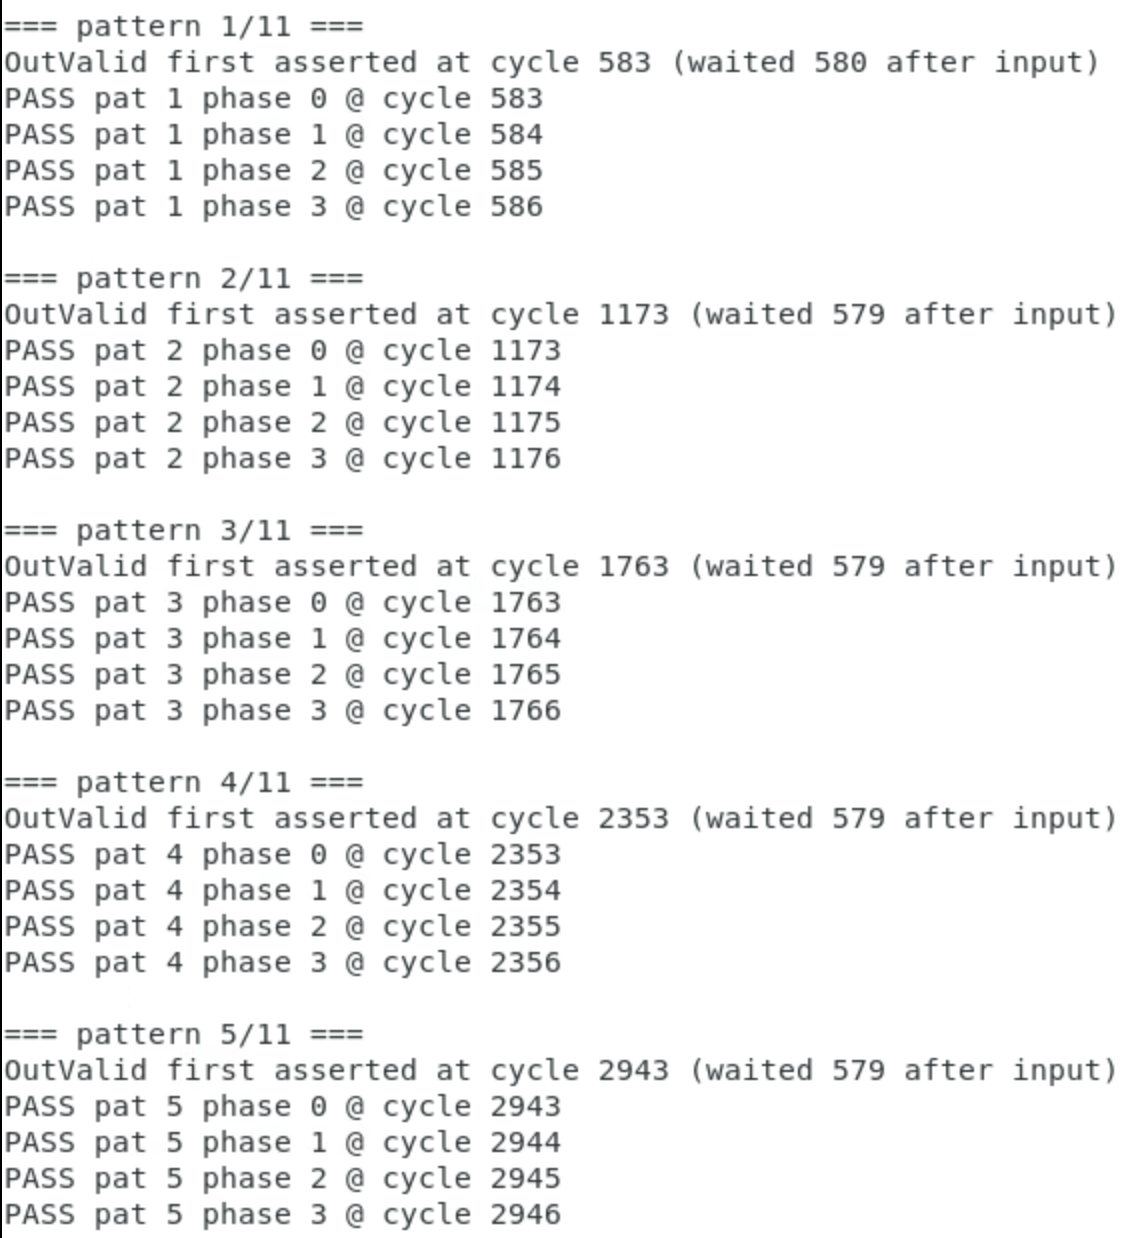
\includegraphics[width=0.69\textwidth]{log1.png}
    \end{subfigure}
    \begin{subfigure}[b]{0.69\textwidth}
        \centering
        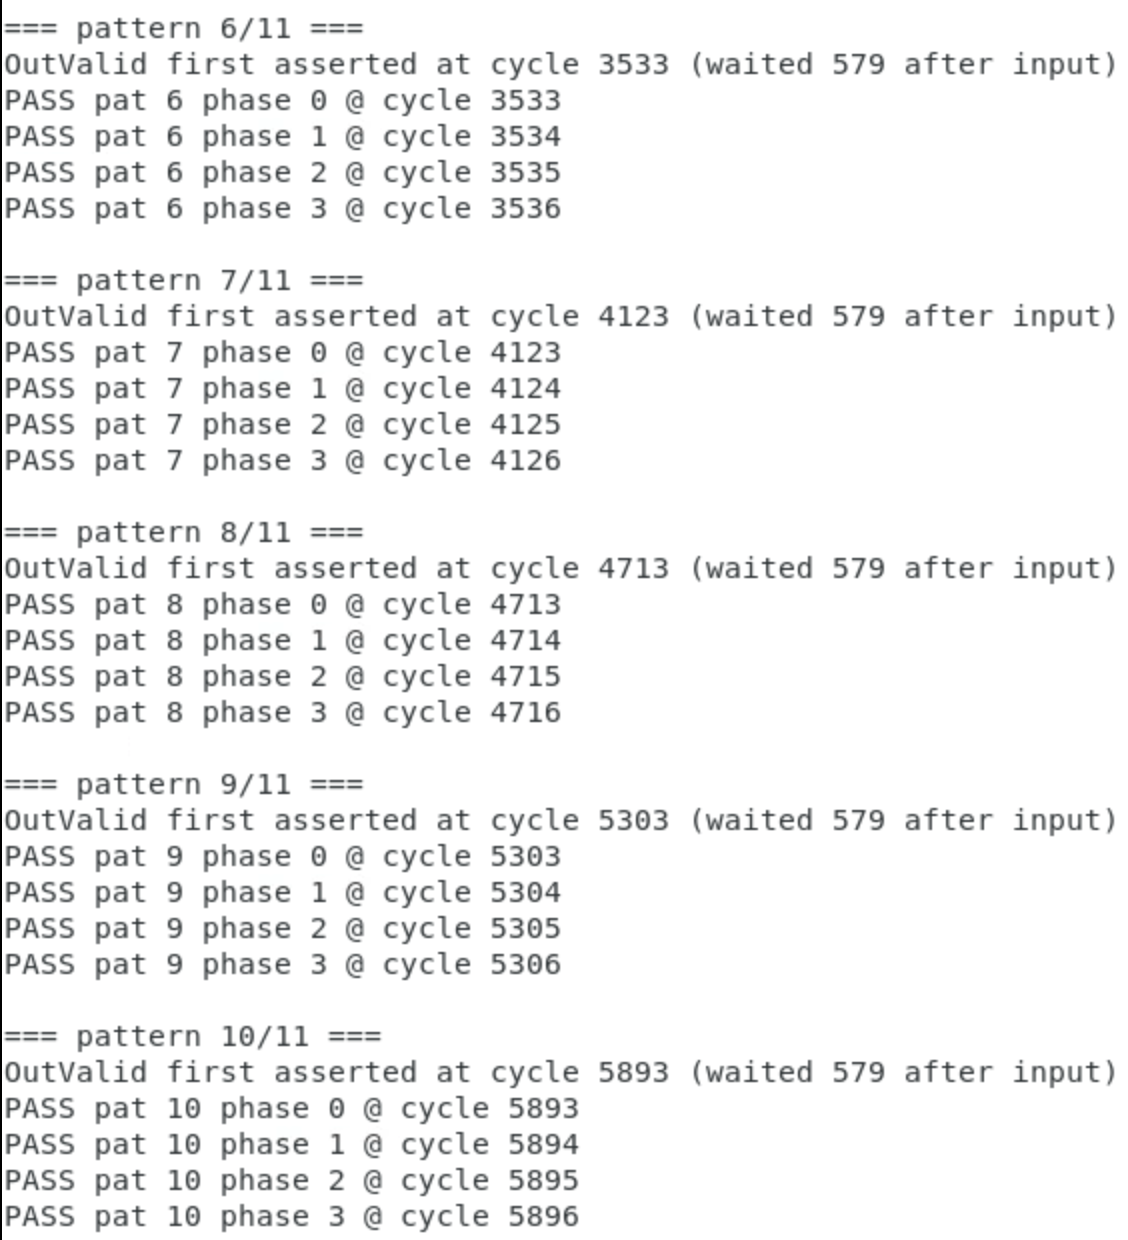
\includegraphics[width=0.69\textwidth]{log2.png}
    \end{subfigure}
    \begin{subfigure}[b]{0.69\textwidth}
        \centering
        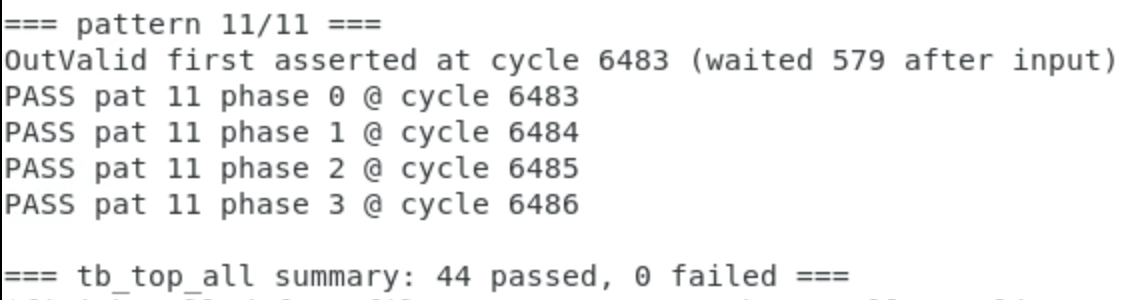
\includegraphics[width=0.69\textwidth]{log3.png}
    \end{subfigure}
    \caption{Simulation log of \texttt{tb\_top\_all.v}}
    \label{fig:tb_top_all_simulation_log}
\end{figure}
\newpage
\subsection{Complete GLS Waveform}
\begin{figure}[htbp]
    \begin{subfigure}[b]{\textwidth}
        \centering
        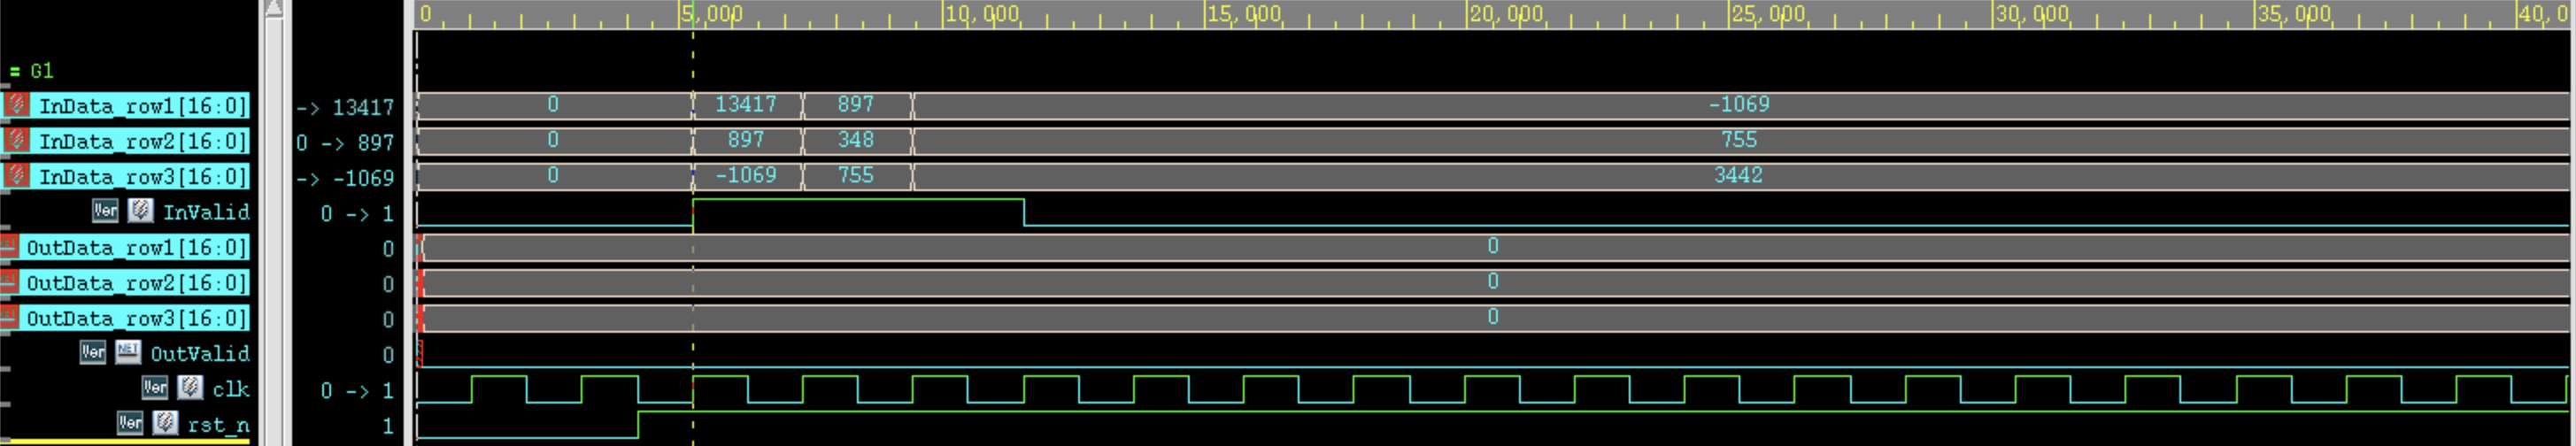
\includegraphics[width=\textwidth]{all_timing_1.png}
    \end{subfigure}
    \begin{subfigure}[b]{\textwidth}
        \centering
        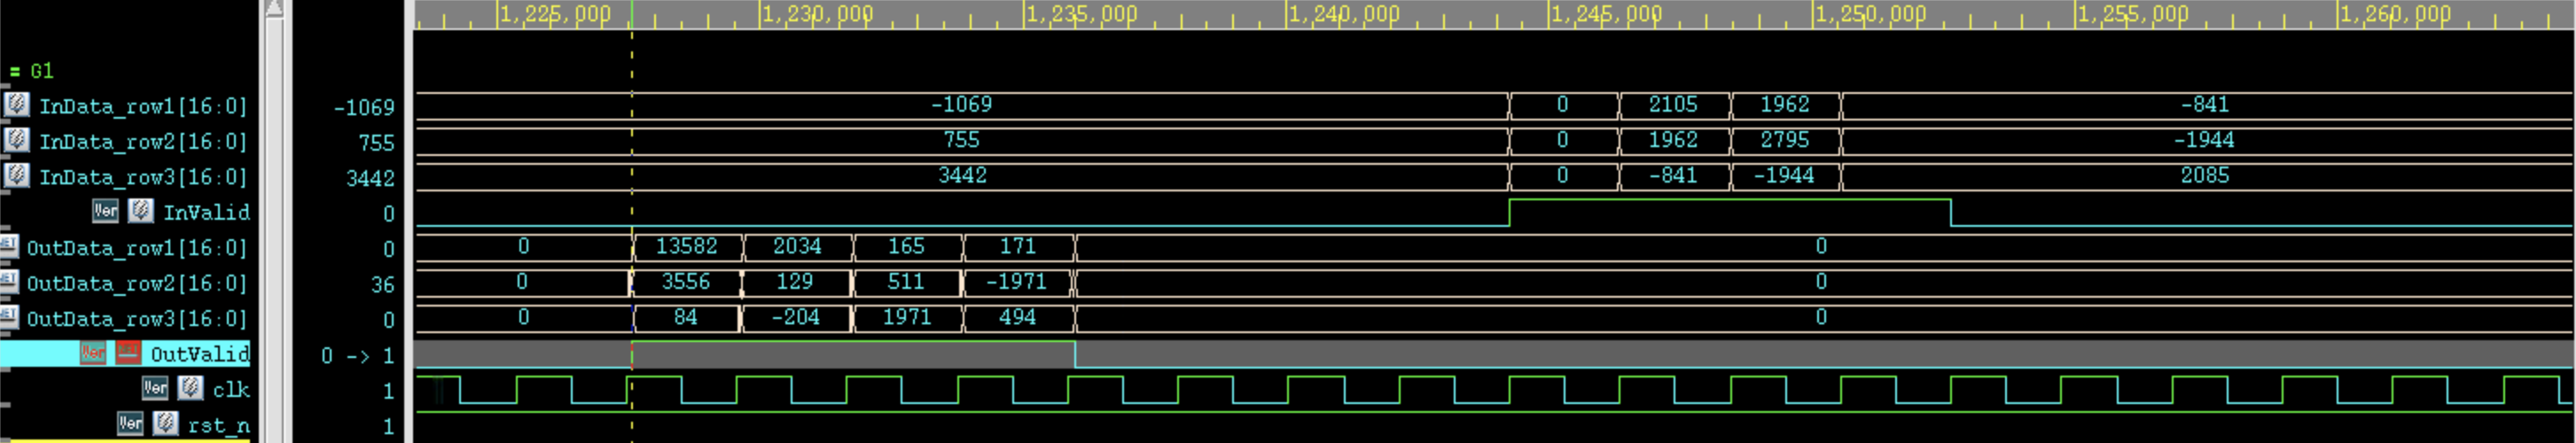
\includegraphics[width=\textwidth]{all_timing_2.png}
    \end{subfigure}
    \begin{subfigure}[b]{\textwidth}
        \centering
        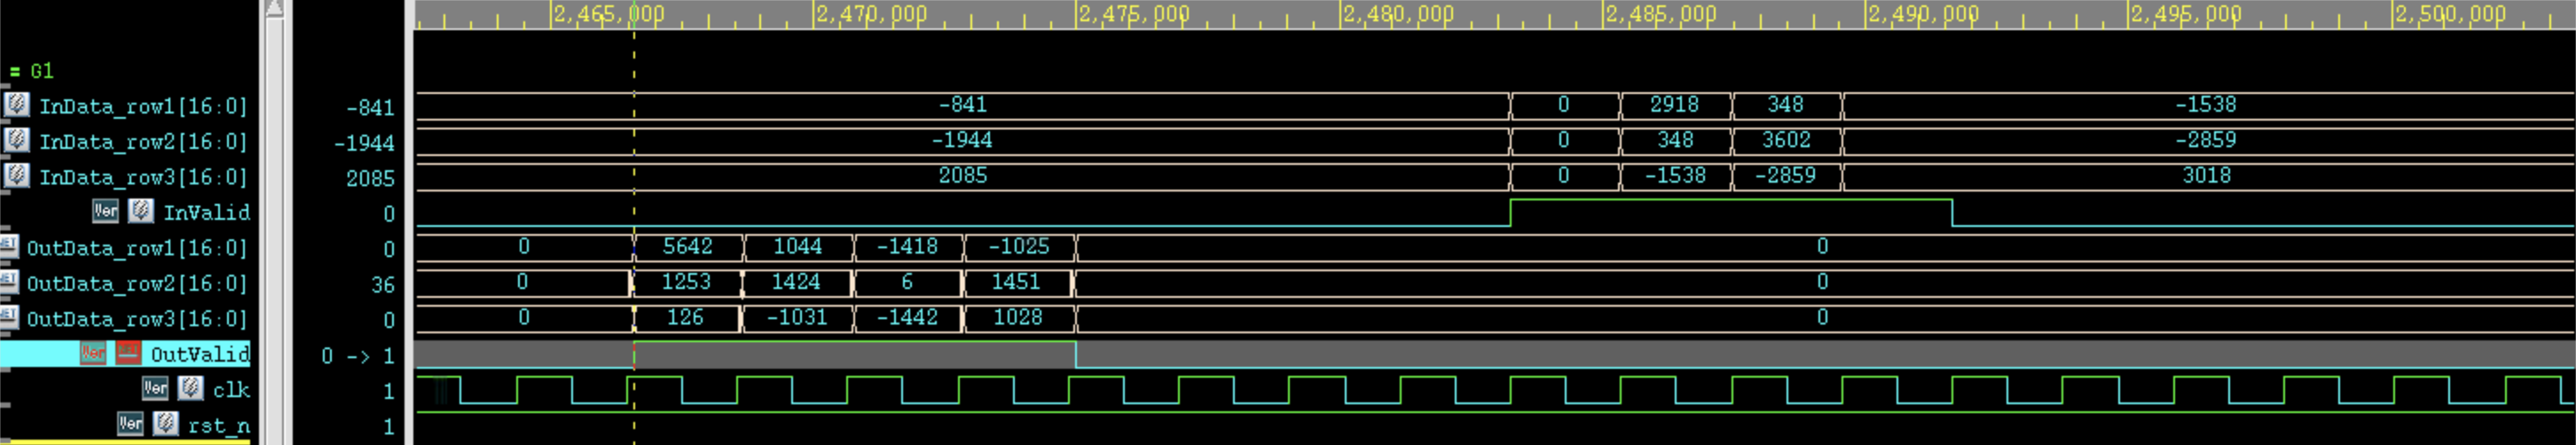
\includegraphics[width=\textwidth]{all_timing_3.png}
    \end{subfigure}
    \begin{subfigure}[b]{\textwidth}
        \centering
        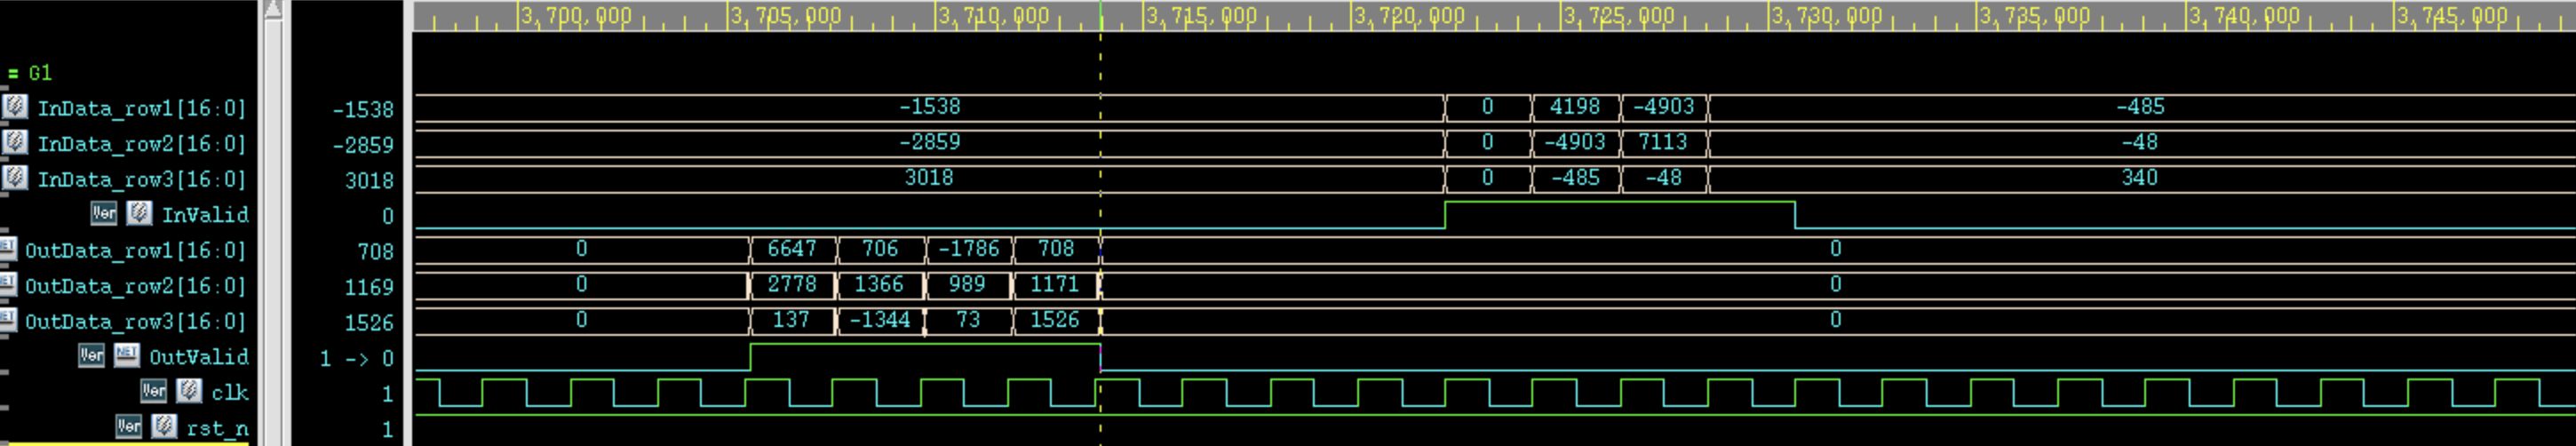
\includegraphics[width=\textwidth]{all_timing_4.png}
    \end{subfigure}
    \begin{subfigure}[b]{\textwidth}
        \centering
        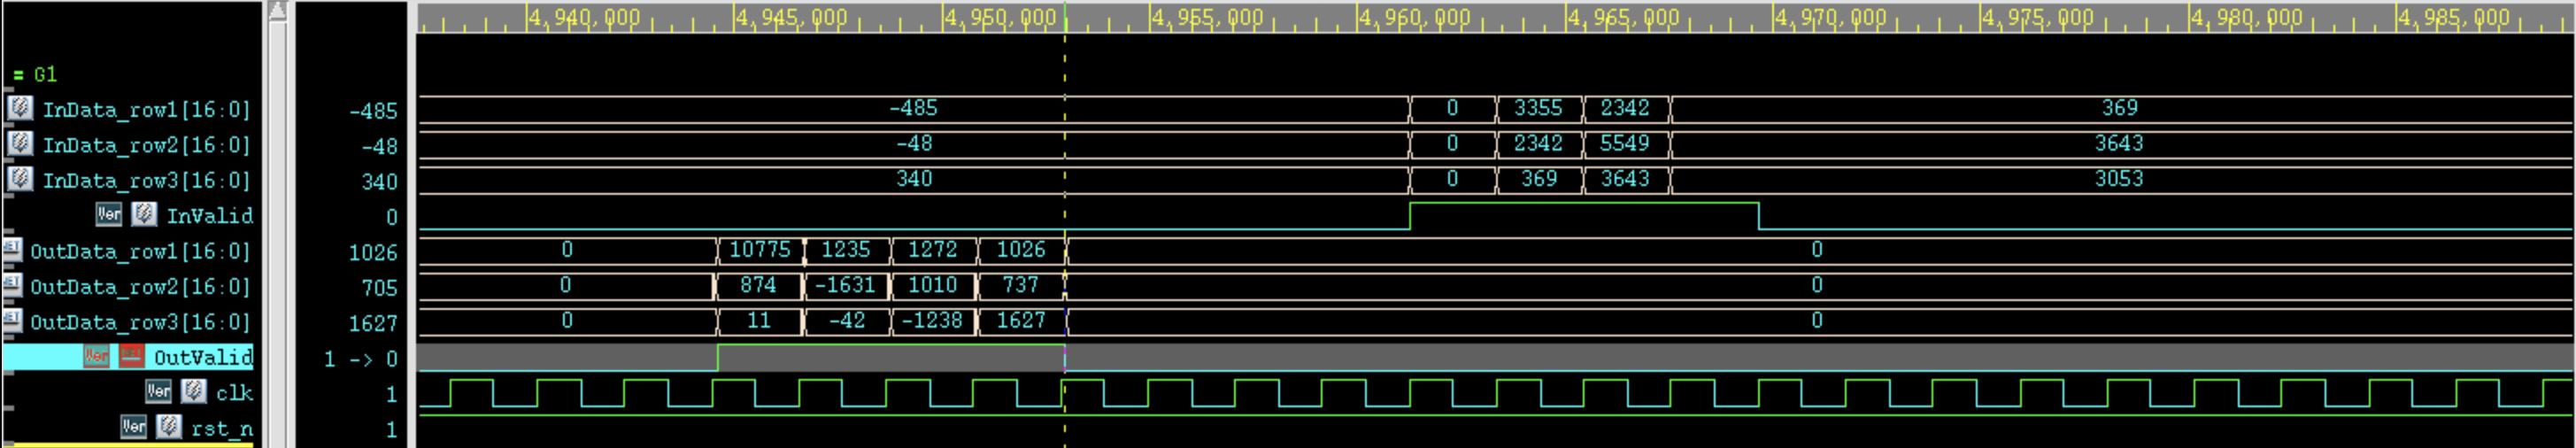
\includegraphics[width=\textwidth]{all_timing_5.png}
    \end{subfigure}
    \begin{subfigure}[b]{\textwidth}
        \centering
        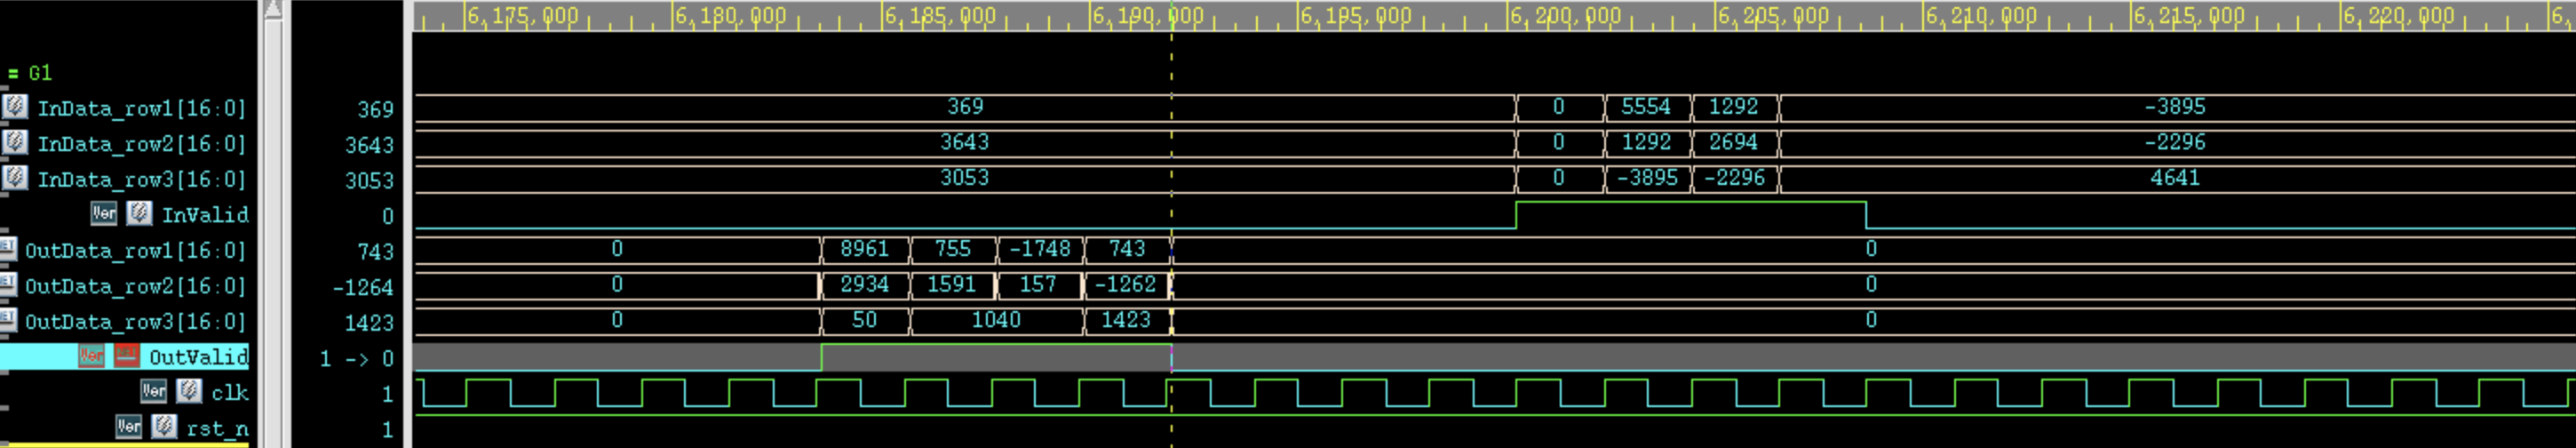
\includegraphics[width=\textwidth]{all_timing_6.png}
    \end{subfigure}
    
\end{figure}

\begin{figure}[htbp]
    \begin{subfigure}[b]{\textwidth}
        \centering
        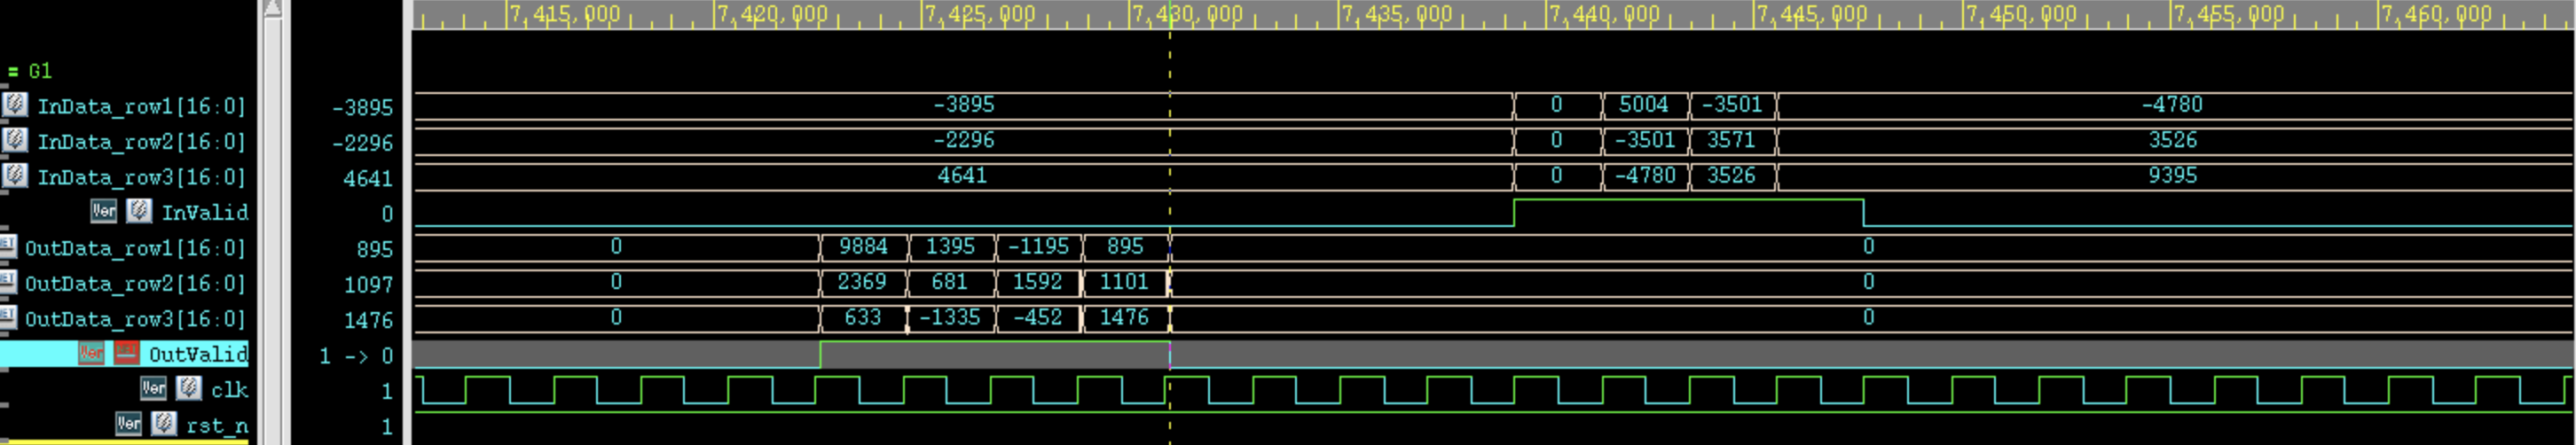
\includegraphics[width=\textwidth]{all_timing_7.png}
    \end{subfigure}
    \begin{subfigure}[b]{\textwidth}
        \centering
        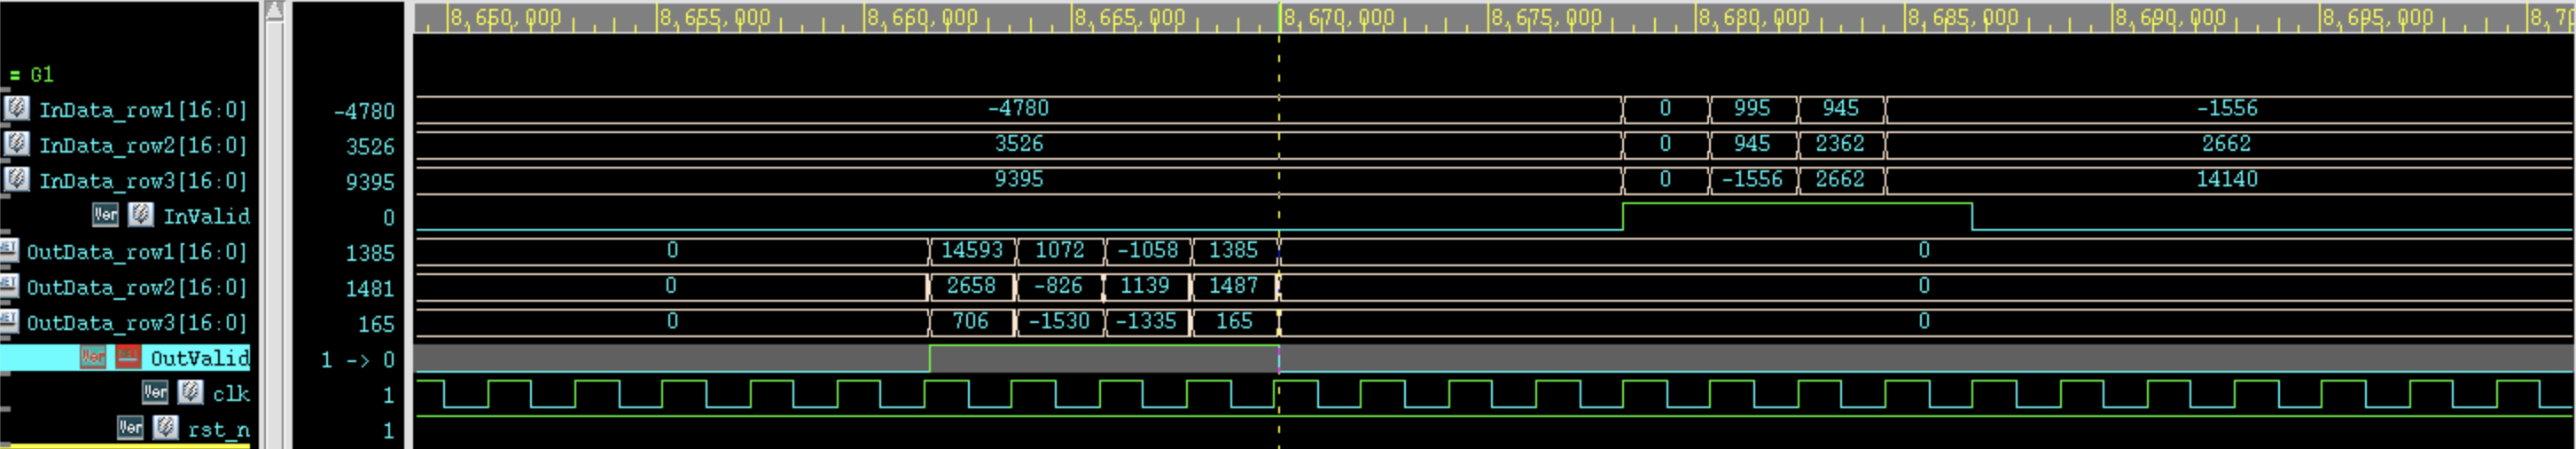
\includegraphics[width=\textwidth]{all_timing_8.png}
    \end{subfigure}
    \begin{subfigure}[b]{\textwidth}
        \centering
        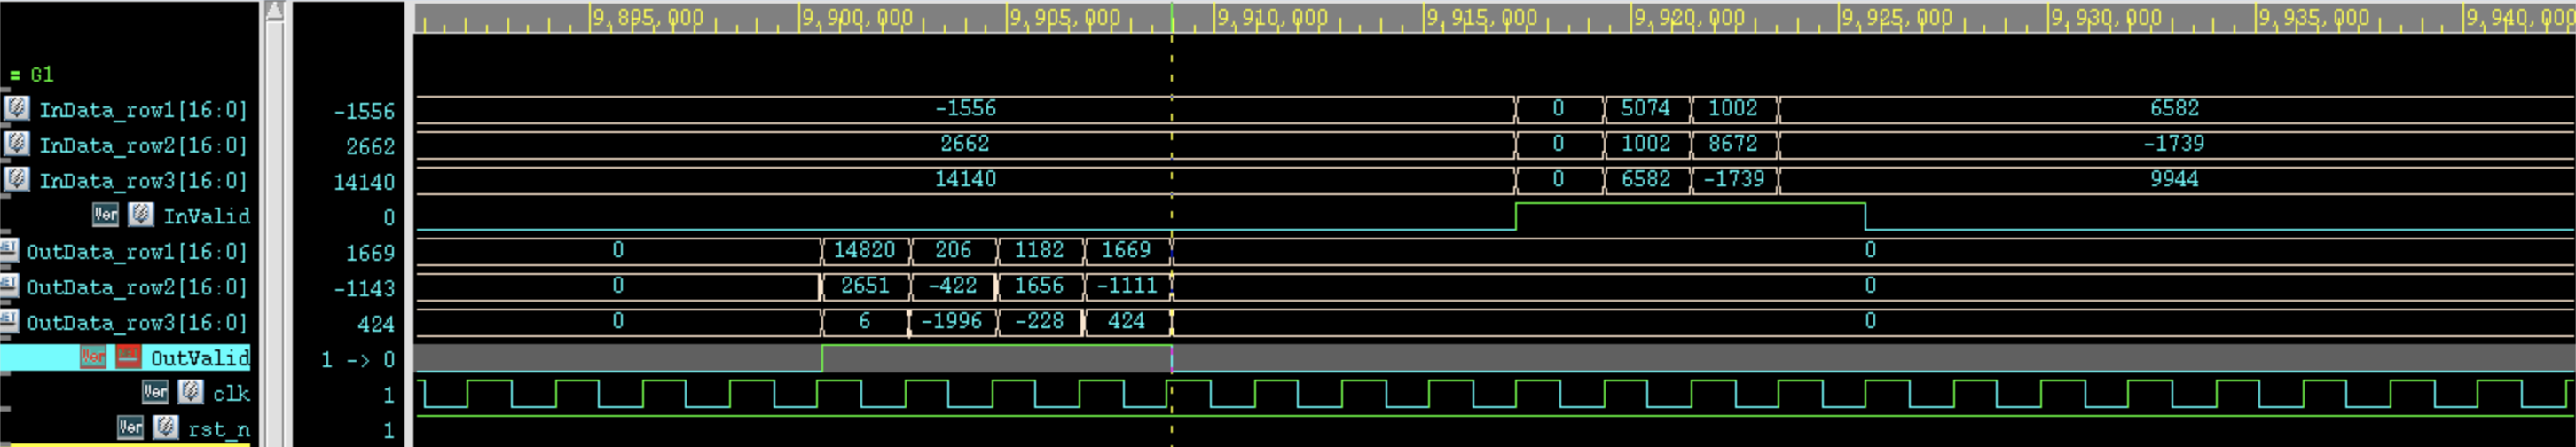
\includegraphics[width=\textwidth]{all_timing_9.png}
    \end{subfigure}
    \begin{subfigure}[b]{\textwidth}
        \centering
        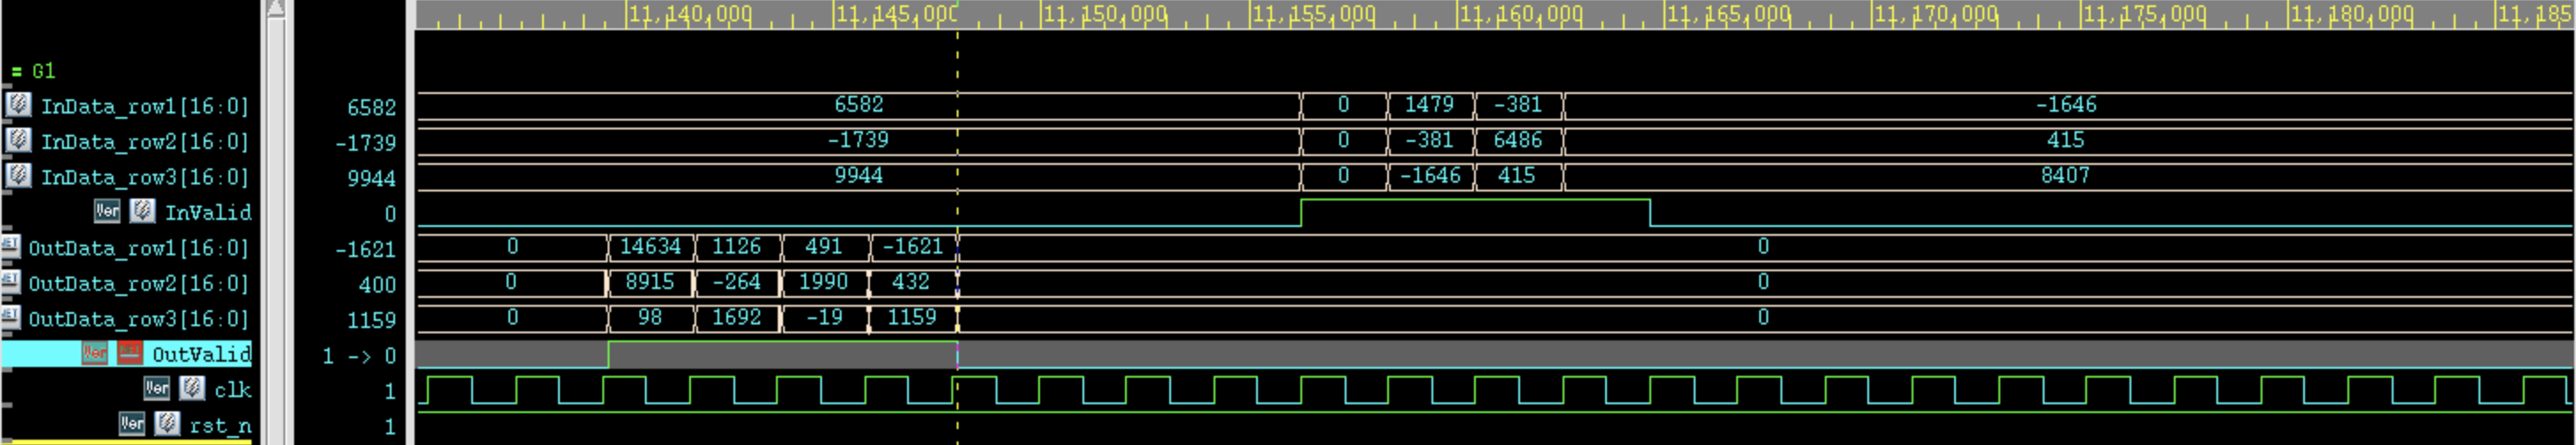
\includegraphics[width=\textwidth]{all_timing_10.png}
    \end{subfigure}
    \begin{subfigure}[b]{\textwidth}
        \centering
        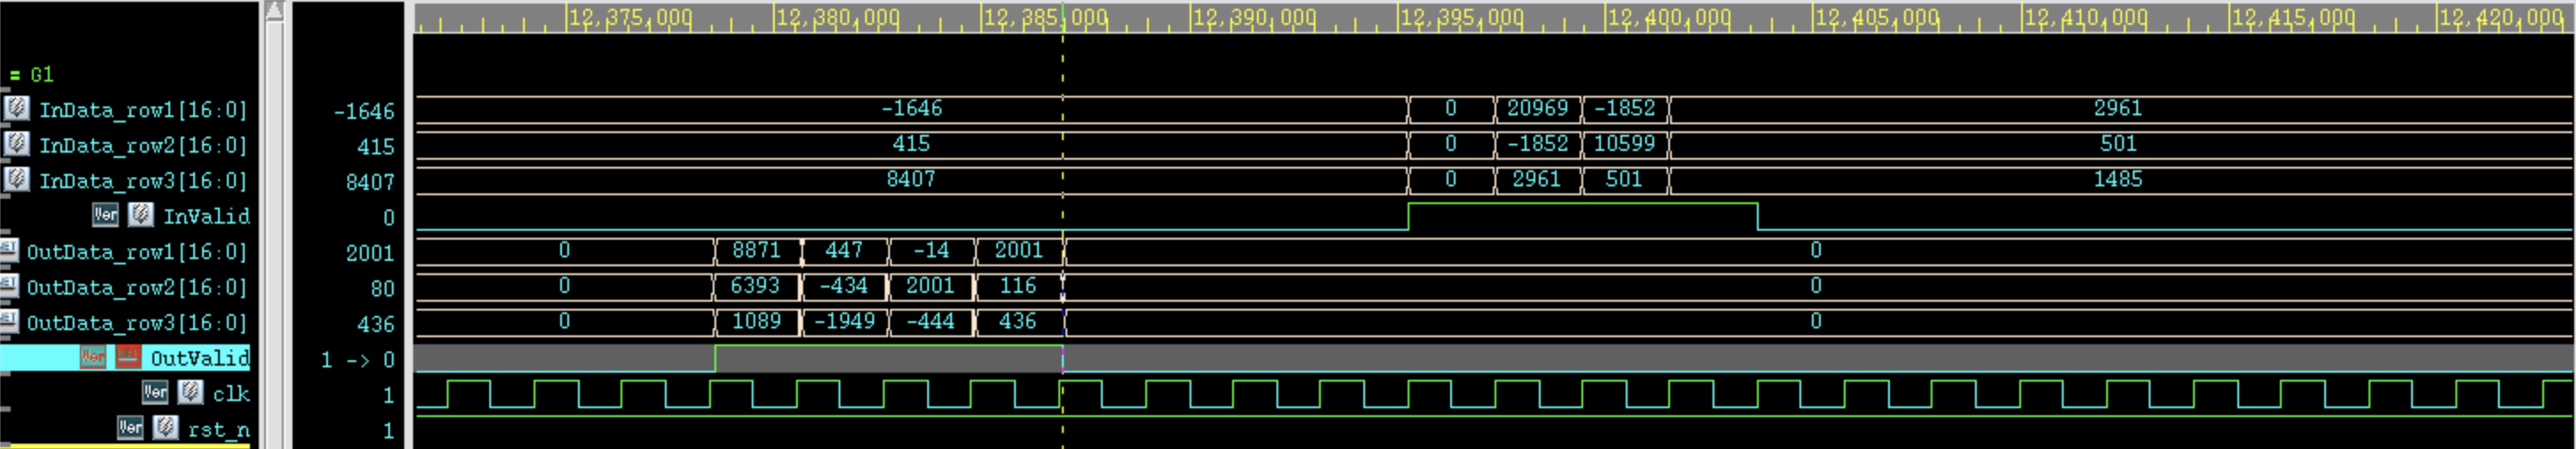
\includegraphics[width=\textwidth]{all_timing_11.png}
    \end{subfigure}
    \begin{subfigure}[b]{\textwidth}
        \centering
        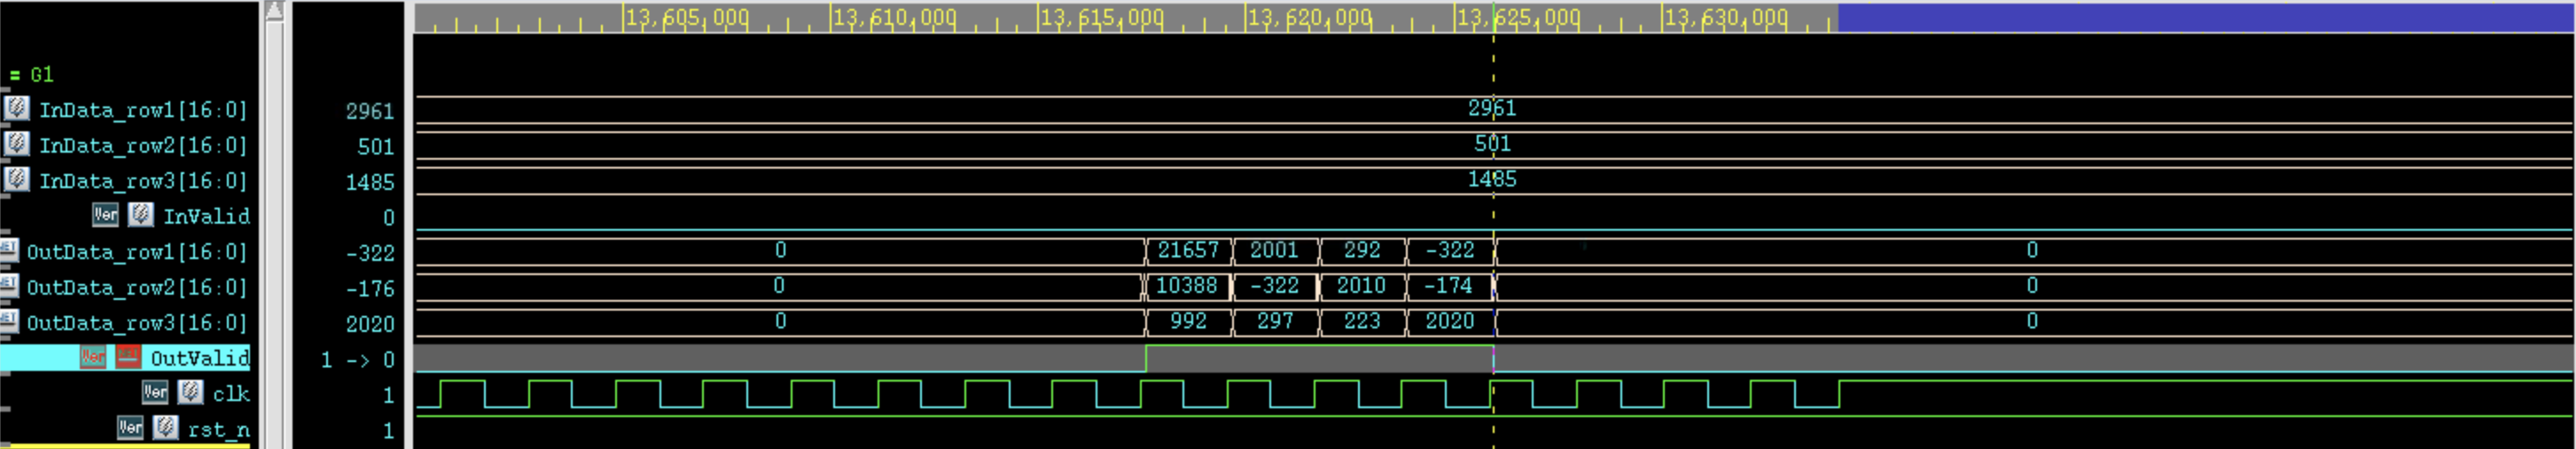
\includegraphics[width=\textwidth]{all_timing_12.png}
    \end{subfigure}
    \caption{Complete GLS timing waveform of \texttt{tb\_top\_all.v}.}
    \label{fig:all_gls_waveform}
\end{figure}
\newpage
\subsection{Timing Report}
\begin{figure}[htbp]
    \begin{subfigure}[b]{0.98\textwidth}
        \centering
        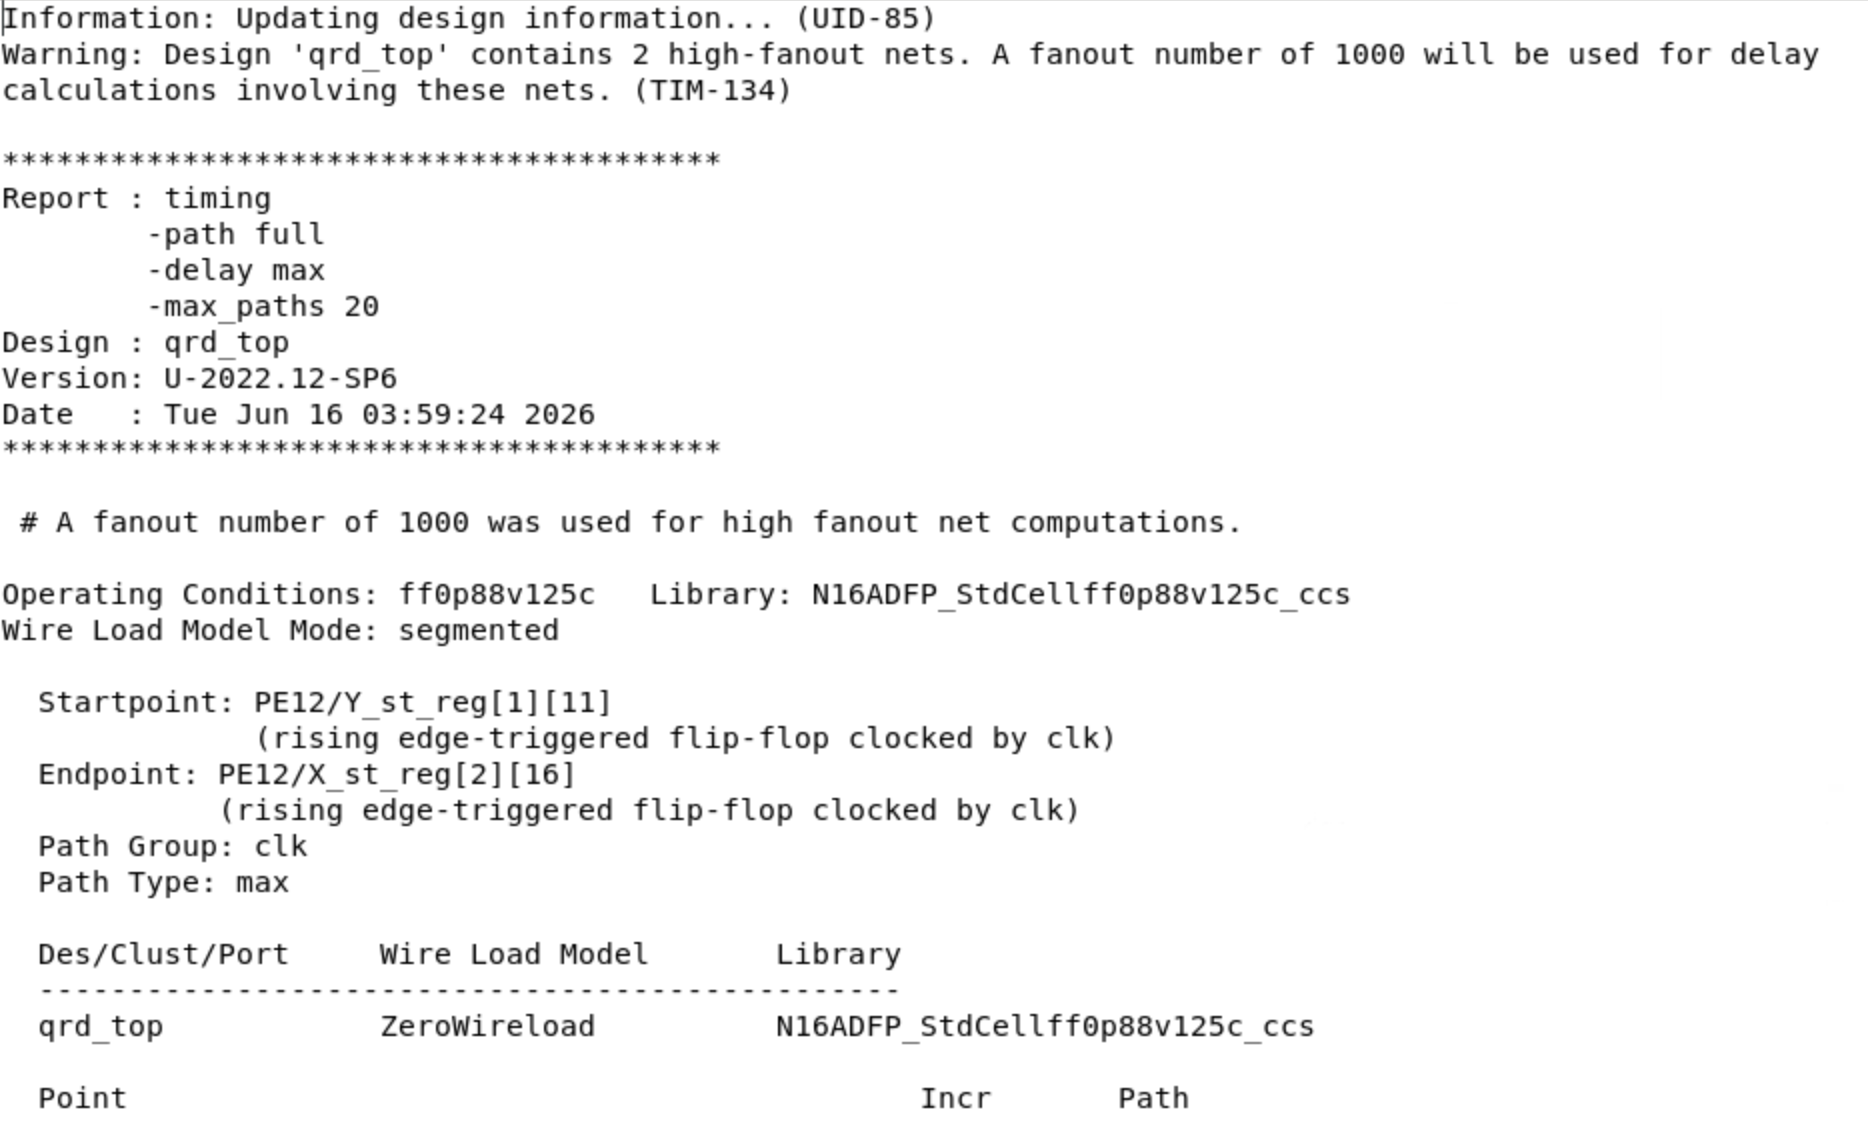
\includegraphics[width=0.98\textwidth]{timing_1.png}
    \end{subfigure}
    \begin{subfigure}[b]{0.98\textwidth}
        \centering
        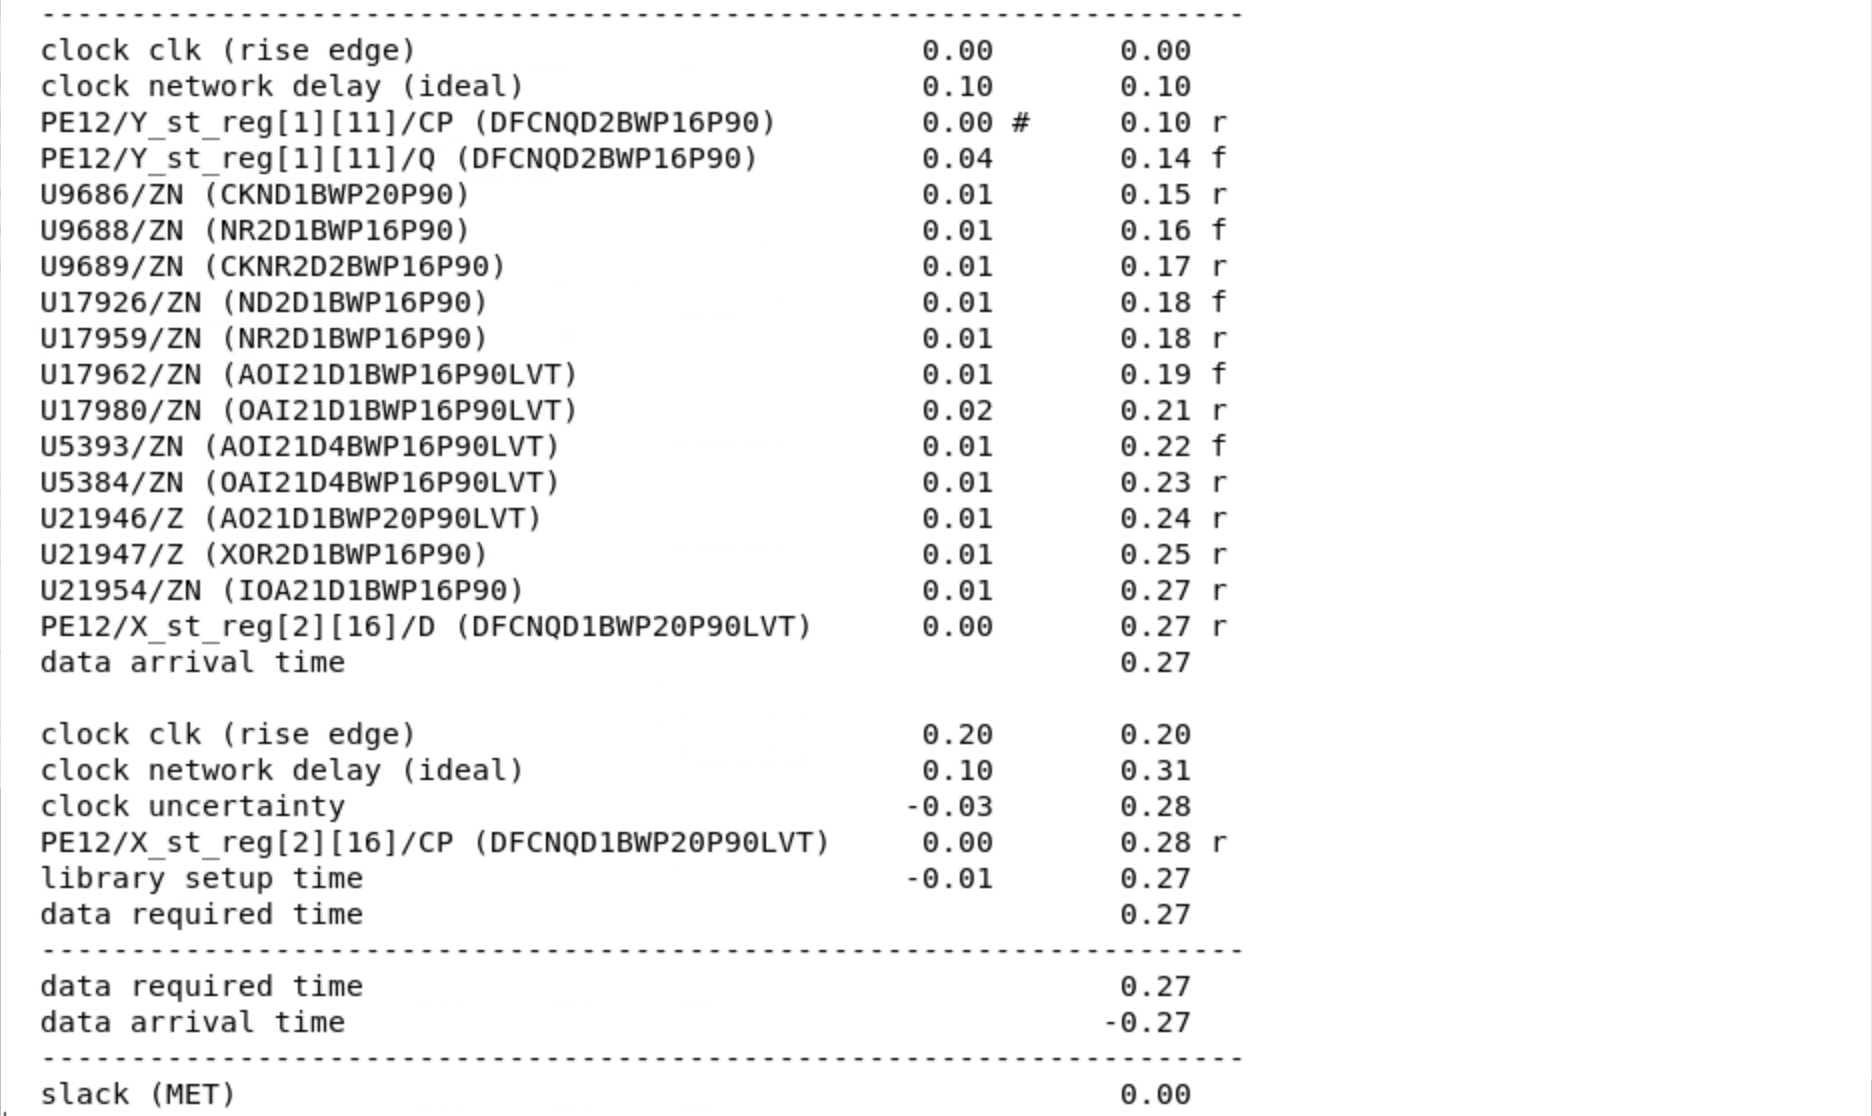
\includegraphics[width=0.98\textwidth]{timing_2.png}
    \end{subfigure}
    \caption{Timing report of \texttt{qrd\_top}.}
    \label{fig:timing_report}
\end{figure}
\newpage
\subsection{Area Report}
\begin{figure}[htbp]
    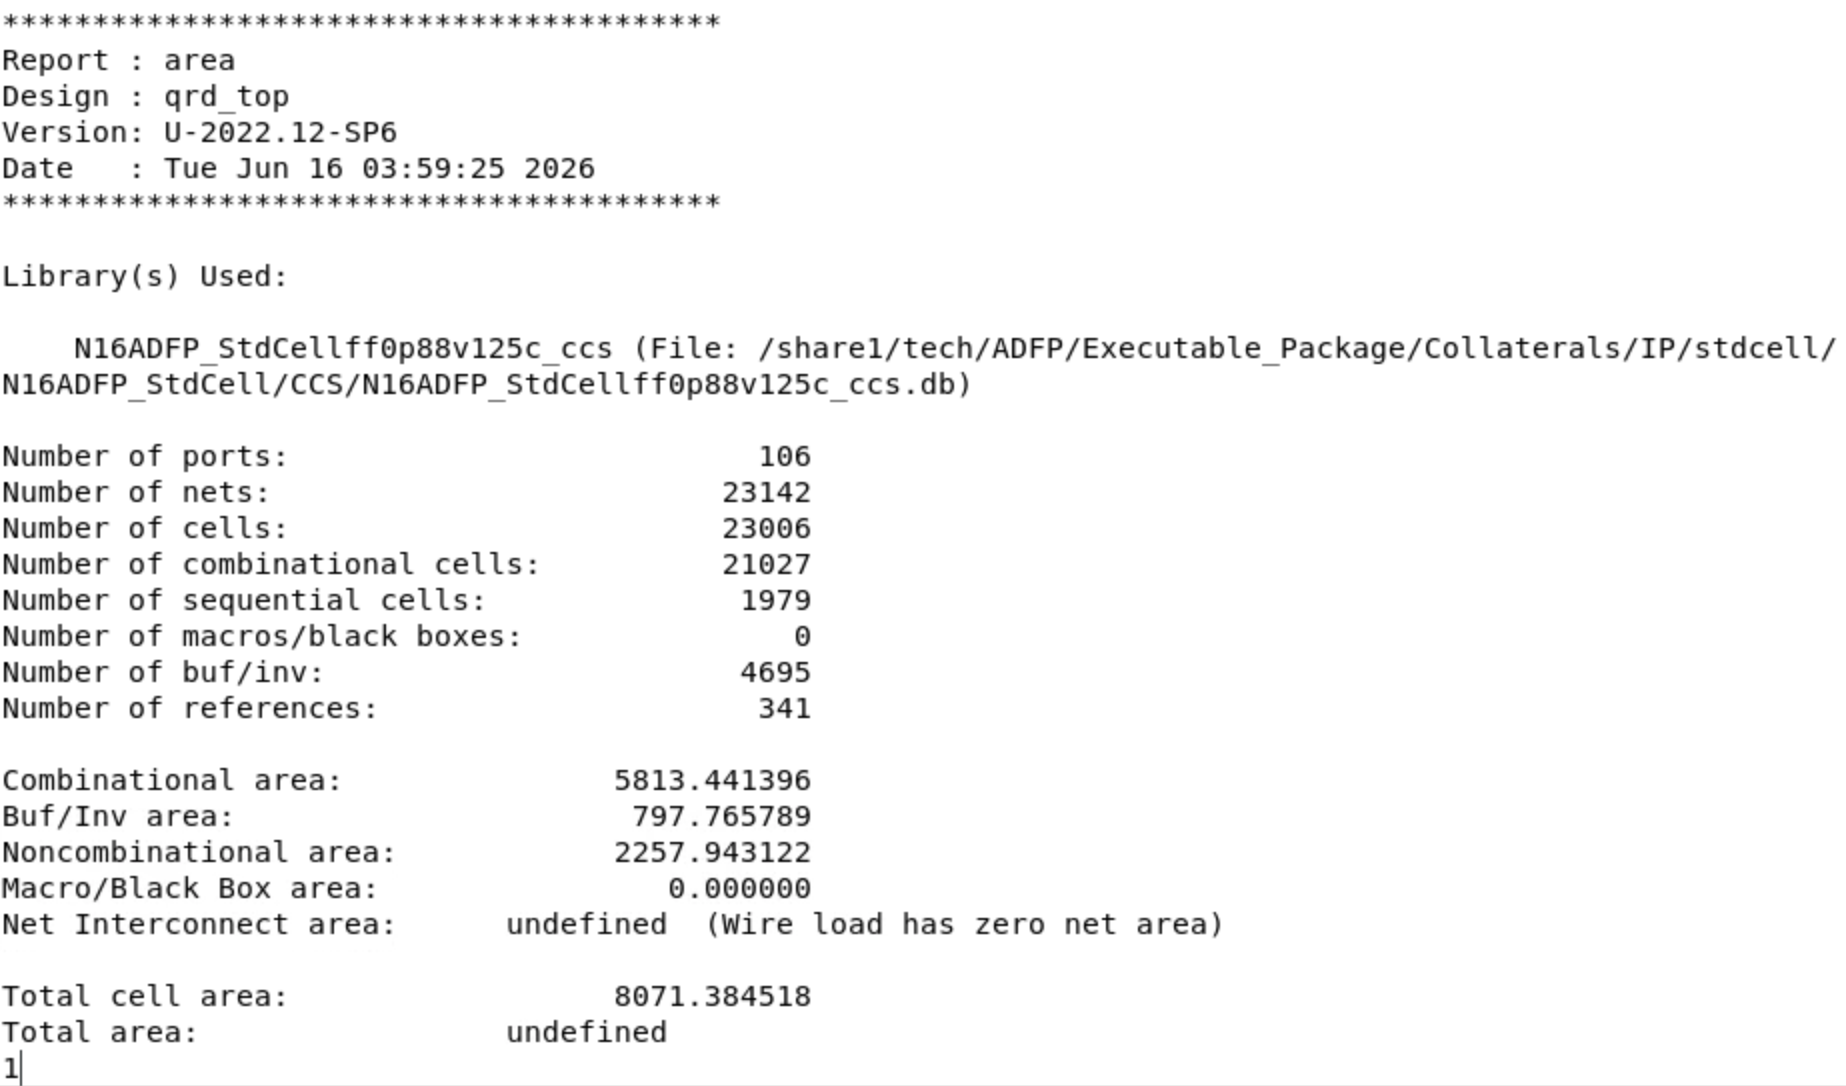
\includegraphics[width=\textwidth]{area.png}
    \caption{Area report of \texttt{qrd\_top}.}
    \label{fig:area_report}
\end{figure}
\end{document}